\providecommand{\econtexRoot}{}
\renewcommand{\econtexRoot}{.}
\providecommand{\econtex}{\econtexRoot/texmf-local/tex/latex/econtex}
\providecommand{\econtexSetup}{\econtexRoot/texmf-local/tex/latex/econtexSetup}
\providecommand{\econtexShortcuts}{\econtexRoot/texmf-local/tex/latex/econtexShortcuts}
\providecommand{\econtexBibMake}{\econtexRoot/texmf-local/tex/latex/econtexBibMake}
\providecommand{\econtexBibStyle}{\econtexRoot/texmf-local/bibtex/bst/econtex}
\providecommand{\notes}{\econtexRoot/texmf-local/tex/latex/handout}
\providecommand{\handoutSetup}{\econtexRoot/texmf-local/tex/latex/handoutSetup}
\providecommand{\handoutShortcuts}{\econtexRoot/texmf-local/tex/latex/handoutShortcuts}
\providecommand{\handoutBibMake}{\econtexRoot/texmf-local/tex/latex/handoutBibMake}
\providecommand{\handoutBibStyle}{\econtexRoot/texmf-local/bibtex/bst/handout}

  
\documentclass[titlepage]{\econtex}\providecommand{\texname}{BufferStockTheory}


\providecommand{\EqDir}{Equations}
\providecommand{\FigDir}{Figures} 
\renewcommand{\FigDir}{Code/Python/Figures}
\providecommand{\CodeDir}{Code}
\providecommand{\CalibrationDir}{Calibration}
\providecommand{\TableDir}{Tables}
\providecommand{\ApndxDir}{Appendices}

\usepackage{subfiles}

\providecommand{\onlyinsubfile}{}
\providecommand{\notinsubfile}{}
\renewcommand{\onlyinsubfile}[1]{}
\renewcommand{\notinsubfile}[1]{#1} 


\usepackage{\econtexSetup}\usepackage{\econtexShortcuts}\usepackage{makecell} 

\provideboolean{Shorter}
\setboolean{Shorter}{true}
\setboolean{Shorter}{false}
\providecommand{\ShorterYN}{\ifthenelse{\boolean{Shorter}}}
\usepackage{rotating}\usepackage{subfigure}


\hypersetup{pdfauthor={Christopher D. Carroll <ccarroll@jhu.edu>},
            pdftitle={Theoretical Foundations of Buffer Stock Saving},
            pdfkeywords={Precautionary saving, buffer-stock saving, consumption, marginal propensity to consume, permanent income hypothesis},
            pdfcreator = {ccarroll@jhu.edu}
}

\begin{document}\bibliographystyle{\econtexBibStyle}
\renewcommand{\onlyinsubfile}[1]{}\renewcommand{\notinsubfile}[1]{#1} 

\hfill{\tiny \texname.tex, \today}

\begin{verbatimwrite}{\texname.title}
Theoretical Foundations of Buffer Stock Saving
\end{verbatimwrite}


\title{Theoretical Foundations of \\ Buffer Stock Saving}

\author{Christopher D. Carroll\authNum}

\keywords{Precautionary saving, buffer stock saving, marginal propensity to consume, permanent income hypothesis}

\jelclass{D81, D91, E21}


\maketitle 


\hypertarget{abstract}{}
\begin{abstract}
This paper builds theoretical foundations for rigorous and intuitive understanding of `buffer stock' saving models, pairing each theoretical result with a quantitative exploration.  After describing conditions under which the consumption function converges, the paper shows that `target' saving behavior, which defines buffer stock saving, arises only under conditions strictly stronger than those that guarantee convergence of the consumption and value functions.  It also shows that average consumption growth equals average income growth in a small open economy populated by buffer stock savers.  Together, the (provided) numerical tools and (proven) analytical results constitute a comprehensive toolkit for understanding buffer stock models.
\end{abstract}

\begin{small}
\parbox{\textwidth}{
\begin{center}
\begin{tabbing}
\texttt{~Archive:~} \= \= \url{http://econ.jhu.edu/people/ccarroll/BufferStockTheory.zip} \kill \\  %
\texttt{~~~~~PDF:~} \> \> \url{http://econ.jhu.edu/people/ccarroll/papers/BufferStockTheory.pdf} \\
\texttt{~~Slides:~} \> \> \url{http://econ.jhu.edu/people/ccarroll/papers/BufferStockTheory-Slides.pdf} \\
\texttt{~~~~~Web:~} \> \> \url{http://econ.jhu.edu/people/ccarroll/papers/BufferStockTheory/}    \\
\texttt{~~GitHub:~} \> \> \url{http://github.com/llorracc/BufferStockTheory} \\
\texttt{~~~~~~~~~~} \> \> \textit{(In GitHub repo, see \texttt{/Code} for tools for solving and simulating the model)} \\
\end{tabbing}
\end{center}
          
\href{https://colab.research.google.com/github/llorracc/BufferStockTheory/blob/master/Code/Python/BufferStockTheory.ipynb}{CLICK HERE} for an interactive \href{https://en.wikipedia.org/wiki/Project\_Jupyter\#Jupyter_Notebook}{Jupyter Notebook} that uses the \href{https://econ-ark/HARK}{Econ-ARK/HARK} toolkit to produce all of the paper's figures (warning: it may take several minutes to launch)}
\end{small}

\begin{authorsinfo}
\name{Contact: \href{mailto:ccarroll@jhu.edu}{\texttt{ccarroll@jhu.edu}}, Department of Economics, 590 Wyman Hall, Johns Hopkins University, Baltimore, MD 21218, \url{http://econ.jhu.edu/people/ccarroll}, and National Bureau of Economic Research.}
\end{authorsinfo}

\thanks{All numerical results herein were produced using the \href{https://econ-ark/HARK}{Econ-ARK/HARK} toolkit, which can be cited as in our references (\cite{carroll_et_al-proc-scipy-2018}); for further reference options see \href{https://econ-ark.org/acknowledging/}{Acknowleding Econ-ARK}.      Thanks to James Feigenbaum, Joseph Kaboski, Miles Kimball, Qingyin Ma, Misuzu Otsuka, Damiano Sandri, John Stachurski, Adam Szeidl, Metin Uyanik, Weifeng Wu,
  and Jiaxiong Yao for comments on earlier versions of this paper, John Boyd for help
  in applying his weighted contraction mapping theorem, Ryoji
  Hiraguchi for extraordinary mathematical insight that improved the
  paper greatly, David Zervos for early guidance to the literature,
  and participants in a seminar at Johns Hopkins University and a
  presentation at the 2009 meetings of the Society of Economic
  Dynamics for their insights.}

\titlepagefinish


\newtheorem{defn}{Definition}
\newtheorem{theorem}{Theorem}

\hypertarget{Introduction}{}
\section{Introduction}

\label{sec:intro}


In the presence of empirically realistic transitory and permanent shocks to income \textit{a la} \cite{friedmanATheory}, only one additional ingredient is required to define a testable model of optimal consumption choice: A utility specification.  Quantitative modelers usually assume constant relative risk aversion (CRRA) utility with geometric discounting, because with those choices the model generates results reasonably in accord with the available evidence.

But the theoretical literature has mostly studied models that are more complex -- say, with a liquidity constraint or consumption floor -- because standard contraction mapping theorems (beginning with \cite{bellmanDynamicProgramming} and including those of Stokey et.~al.~\citeyearpar{slpMethods}) cannot be applied when the utility function is unbounded (like CRRA - see the end of \hyperlink{DiffFromLit}{section \ref{subsec:Setup}} for details).\footnote{It is unclear whether newer methods such as those of \cite{mnUnique}) could overcome this problem, or how difficult it would be to do so; but in any case this particular problem does not seem to have been tackled by those methods or any others.}

Numerical solutions to such problems have become widespread following Zeldes~\citeyearpar{zeldesStochastic}, without too much attention to theoretical underpinnings because the conclusions being sought are quantitative.  But without theoretical underpinnings, the `black box' character of numerical solutions makes it difficult to build intuition for how results might change with changes in the structure or calibration of the model.  Indeed, without such theory, it can be difficult even to check whether a computational solution is correct.

For example, numerical solutions typically indicate the existence of a target level of nonhuman wealth (`cash' for short).  Carroll~\citeyearpar{carrollBrookings,carrollBSLCPIH} showed that target saving behavior arises under plausible parameter values for both infinite and finite horizon models.  Gourinchas and Parker~\citeyearpar{gpLifeCycle} estimate that for the mean household, buffer stock behavior characterizes behavior from age 25 until around age 40-45; using the same model with different data Cagetti~\citeyearpar{cagettiWprofiles} finds target saving behavior into the 50s for the median household.  Such target saving plays a key role in understanding the main results of the recent heterogeneous agent macroeconomics literature, including, for example, the insight in \cite{kmpHandbook} that explains why, during the Great Recession, middle-class consumers cut their consumption more than the poor or the rich.  Similar behavior characterizes the `wealthy hand-to-mouth' in \cite{kaplanViolanteWeidner_wealthyH2M}, who have plenty of illiquid assets but liquid assets that are low relative to their target levels.  Despite the centrality of the mechanism, none of these papers provides a characterization of the circumstances under which target saving will emerge. 

The paper's main technical contributions are to articulate the (surprisingly loose) conditions under which the problem defines a contraction mapping with a nondegenerate consumption function, and conditions under which the resulting consumption function a implies expstence of a `target' wealth-to-permanent-income ratio.  (This is the sense in which the paper studies the class of `buffer stock' saving models.)  The key condition required for target saving is that the model's parameters need to satisfy a ``Growth Impatience Condition'' (equation \eqref{eq:GIC}) which relates preferences to the predictable growth rate of income.

The paper also provides analytical foundations for other results that have become familiar from the numerical literature.  All theoretical conclusions are paired with numerically computed illustrations (using an open-source toolkit available from the \href{https://github.com/econ-ark/REMARK/blob/master/REMARKs/BufferStockTheory/BufferStockTheory.ipynb}{Econ-ARK} project).  All of the insights of this paper are instantiated in the toolkit, which algorithmically flags parametric choices under which a problem fails to define a contraction mapping, under which a target level of wealth does not exist, or under which the solution is otherwise degenerate.

The paper proceeds in three parts.

The first part articulates the conditions required for the problem to define a unique nondegenerate limiting consumption function, and discusses the relation of the paper's model to models previously considered in the literature.  The required conditions turn out to be interestingly parallel to those required for the liquidity constrained perfect foresight model; that parallel is explored and explained.  Next, the paper derives some limiting properties of the consumption function as cash approaches infinity and as it approaches its lower bound, and the theorem is proven explaining when the problem defines a contraction mapping.  Finally, a related class of commonly-used models (exemplified by Deaton~\citeyearpar{deatonLiqConstr}) is shown to constitute a particular limit of this paper's more general model.

The \hyperlink{AnalysisoftheConvergedConsumptionFunction}{next section} examines five key properties of the model. First, as \hyperlink{LimitsAsmtToInfty}{cash approaches infinity} the expected growth rate of consumption and the marginal propensity to consume (MPC) converge to their values in the perfect foresight case. Second, as \hyperlink{LimitsAsmtToZero}{cash approaches zero} the expected growth rate of consumption approaches infinity, and the MPC approaches a simple analytical limit.  Third, if the consumer is `growth impatient,' a \hyperlink{onetarget}{unique target cash-to-permanent-income ratio} will exist.  Fourth, at the target cash ratio, the \hyperlink{cGroLTpGro}{expected growth rate of consumption} is slightly less than the expected growth rate of permanent noncapital income.  Finally, the expected growth rate of consumption \hyperlink{dcgdxneg}{is declining in the level of cash}. The first four propositions are proven under general assumptions about parameter values; the last is shown to hold if there are no transitory shocks, but may fail in extreme cases if there are both transitory and permanent shocks.

Szeidl~\citeyearpar{szeidlInvariant} has shown that such an economy will be characterized by stable invariant distributions for the consumption ratio, the wealth ratio, and other variables.\footnote{Szeidl's proof supplants the analysis in an earlier draft of this paper, which conjectured that such a result held and provided supportive simulation evidence.}  Using Szeidl's result, the final section discusses conditions under which, even with a fixed aggregate interest rate that differs from the time preference rate, an economy populated by buffer stock consumers converges to a balanced growth equilibrium in which the growth rate of consumption tends toward the (exogenous) growth rate of permanent income.

\hypertarget{The-Problem}{}
\section{The Problem}

\subsection{Setup}
\label{subsec:Setup}

The consumer solves an optimization problem from period
$t$ until the end of life at $T$ defined by the objective
\begin{verbatimwrite}{\EqDir/supfn.tex}
\begin{eqnarray}
  \label{eq:supfn}
  \max~ \Ex_{t}\left[\sum_{n=0}^{T-t} \DiscFac^{n} \uFunc(\cLevBF_{t+n})\right]
\end{eqnarray}
\end{verbatimwrite}
\begin{eqnarray}
  \label{eq:supfn}
  \max~ \Ex_{t}\left[\sum_{n=0}^{T-t} \DiscFac^{n} \uFunc(\cLevBF_{t+n})\right]
\end{eqnarray}

where
$\uFunc(\bullet)=\bullet^{1-\CRRA}/(1-\CRRA)$ is a constant relative
risk aversion utility function with $\CRRA > 1$.\footnote{The main
  results also hold for logarithmic utility which is the limit as
  $\CRRA \rightarrow 1$ but incorporating the logarithmic special case
  in the proofs is cumbersome and therefore
  omitted.}$^{,}$\footnote{We will define the infinite horizon
  solution as the limit of the finite horizon problem as the horizon
  $T-t$ approaches infinity.}  The consumer's initial condition is
defined by market resources $\mLevBF_{t}$ (\cite{deatonLiqConstr}
called this `cash-on-hand') and permanent noncapital income $\pLevBF_{t}$.

In the usual treatment, a dynamic budget constraint (DBC) simultaneously incorporates
all of the elements that determine next period's $\mLevBF$ given this
period's choices; but for the detailed analysis here, it will be useful to
disarticulate the steps so that individual ingredients can be separately examined:

\begin{verbatimwrite}{\EqDir/DBCparts.tex}
\begin{eqnarray}
\aLevBF_{t}   &=&\mLevBF_{t}-\cLevBF_{t}  \label{eq:DBCparts} \\
\bLevBF_{t+1}   & = & \aLevBF_{t} \Rfree \notag \\
\pLevBF_{t+1} &=&\pLevBF_{t} \underbrace{\PGro\pShk_{t+1}}_{\equiv \PGro_{t+1}}  \notag \\
\mLevBF_{t+1} &=& \bLevBF_{t+1} +\pLevBF_{t+1}\tShkAll_{t+1},  \notag
\end{eqnarray}
\end{verbatimwrite}
\begin{eqnarray}
\aLevBF_{t}   &=&\mLevBF_{t}-\cLevBF_{t}  \label{eq:DBCparts} \\
\bLevBF_{t+1}   & = & \aLevBF_{t} \Rfree \notag \\
\pLevBF_{t+1} &=&\pLevBF_{t} \underbrace{\PGro\pShk_{t+1}}_{\equiv \PGro_{t+1}}  \notag \\
%
\mLevBF_{t+1} &=& \bLevBF_{t+1} +\pLevBF_{t+1}\tShkAll_{t+1},  \notag
\end{eqnarray}
 where $\aLevBF_{t}$ indicates the consumer's assets at the end of period $t$, which grow by a fixed interest factor $\Rfree =(1+\rfree)$ between periods,\footnote{See \cite{mstCapIncFluct} for interesting new work that considers the case where capital returns are stochastic and liquidity constraints exist.  \cite{benhabibWealth} examines implications of capital income risk for the distribution of wealth.}  so that $\bLevBF_{t+1}$ is the consumer's financial (`bank') balances before next period's consumption choice;\footnote{Allowing a stochastic interest factor is straightforward but adds little insight.  The effects are more interesting for analysis of the invariant distribution (\cite{szeidlInvariant}).} $\mLevBF_{t+1}$ (`market resources' or `money') is the sum of financial wealth $\bLevBF_{t+1}$ and noncapital income $\pLevBF_{t+1}\tShkAll_{t+1}$ (permanent noncapital income $\pLevBF_{t+1}$ multiplied by a mean-one iid transitory income shock factor $\tShkAll_{t+1}$; from the perspective of period $t$, future transitory shocks are assumed to satisfy $\Ex_{t}[{\tShkAll}_{t+n}]=1~\forall~n\geq 1$). Permanent noncapital income in period $t+1$ is equal to its previous value, multiplied by a growth factor $\PGro$, modified by a mean-one iid shock $\pShk_{t+1}$, $\Ex_{t}[{\pShk}_{t+n}]=1~\forall~n \geq 1$ satisfying $\pShk \in [\ushort{\pShk},\bar{\pShk}]$ for $0 < \ushort{\pShk} \leq 1 \leq \bar{\pShk} < \infty$ where $\ushort{\pShk}=\bar{\pShk}=1$ is the degenerate case with no permanent shocks.\footnote{It is useful to emphasize that permanent noncapital income as defined here differs from what Deaton~\citeyearpar{deatonUnderstandingC} calls permanent income (which is often adopted in the macro literature).  Deaton defines permanent income as the amount that a perfect foresight consumer could spend while leaving total (human and nonhuman) wealth constant.  Relatedly, we refer to $\mLevBF_{t}$ as `cash-on-hand' or `market resources' rather than as wealth to avoid any confusion for readers accustomed to thinking of the discounted value of future noncapital income as a part of wealth.  The `market resources' terminology is motivated by the model's assumption that human wealth cannot be capitalized, an implication of anti-slavery laws.}  (Hereafter for brevity we occasionally drop time subscripts, e.g.\ $\Ex[\pShk^{-\CRRA}]$ signifies $\Ex_{t}[\pShk_{t+1}^{-\CRRA}]$.)



In future periods $t+n ~\forall~ n \geq 1$ there is a small probability $\pZero$ that income will
be zero (a `zero-income event'),
\begin{verbatimwrite}{\EqDir/tShkDef}
\begin{equation}
\tShkAll _{t+n}=
\begin{cases}
 0\phantom{_{t+1}/\pNotZero} & \text{with probability $\pZero>0$} \\
 \tShkEmp_{t+n}/\pNotZero      & \text{with probability $\pNotZero  $} 
\end{cases} \label{eq:tShkDef}
\end{equation}
\end{verbatimwrite}
\begin{equation}
\tShkAll _{t+n}=
\begin{cases}
 0\phantom{_{t+1}/\pNotZero} & \text{with probability $\pZero>0$} \\
 \tShkEmp_{t+n}/\pNotZero      & \text{with probability $\pNotZero  $}
\end{cases} \label{eq:tShkDef}
\end{equation}

where $\tShkEmp_{t+n}$ is an iid mean-one random variable
($\Ex_{t}[{\tShkEmp}_{t+n}]=1~\forall~n>0$)
that has a distribution
satisfying $\tShkEmp \in \lbrack \ushort{\tShkEmp},\bar{\tShkEmp}\rbrack$
where $0<\ushort{\tShkEmp} \leq 1 \leq \bar{\tShkEmp}<\infty$
(degenerately $\ushort{\tShkEmp}=\bar{\tShkEmp}=1$). (See \cite{rabaultBorrowing} and \cite{lsIncFluct} for analyses of cases where the shock processes have unbounded support).  Call the cumulative
distribution functions $\CDF_{\pShk}$ and $\CDF_{\tShkEmp}$ (and $\CDF_{\tShkAll}$
is derived trivially from \eqref{eq:tShkDef} and $\CDF_{\tShkEmp}$).
Permanent income and cash start out strictly positive, $\{\pLevBF_{t},\mLevBF_{t}\} \in
(0,\infty)$, and as usual the consumer cannot die in
debt, so that 
\begin{eqnarray}
  \cLevBF_{T} & \leq & \mLevBF_{T} \label{eq:NoDebtAtDeath}.
\end{eqnarray}

The model looks more special than it is.  In particular, the
assumption of a positive probability of zero-income events may seem
objectionable.  However, it is easy to show that a model with a
nonzero minimum value of $\tShkAll$ (motivated, for example, by the
existence of unemployment insurance) can be redefined by capitalizing
the PDV of minimum income into current market assets,\footnote{So long
  as this PDV is a finite number and unemployment benefits are
  proportional to $\pLevBF_{t}$; see the discussion in
  section~\ref{sec:discussConvergence}.}  analytically transforming
that model back into the model analyzed here.  Also, the assumption of
a positive point mass (as opposed to positive density) for the worst
realization of the transitory shock is inessential, but simplifies the proofs and is a powerful aid to intuition.

\begin{comment}
Combining the transition equations, the recursive nature of
the problem allows us to rewrite it more compactly in Bellman equation form,
\begin{eqnarray*}
\VFunc_{t}(\mLevBF_{t},\pLevBF_{t}) & = & \max_{\cLevBF_{t}}~\left\{\uFunc(\cLevBF_{t})+\DiscFac \Ex_{t}\left[ \VFunc_{t+1}((\mLevBF_{t}-\cLevBF_{t})\Rfree+ \pLevBF_{t+1}\tShkAll_{t+1},\pLevBF_{t} \PGro  \pShk_{t+1})\right]\right\}
.
\end{eqnarray*}
\end{comment}

\hypertarget{DiffWithLit}{} This model differs from Bewley's~\citeyearpar{bewleyPIH} classic formulation in several ways. The CRRA utility function does not satisfy Bewley's assumption that $\uFunc(0)$ is well defined, or that $\uP(0)$ is well defined and finite, so neither the value function nor the marginal value function will be bounded.  It differs from Schectman and Escudero~\citeyearpar{seIncFluct} in that they impose liquidity constraints and positive minimum income.  It differs from both of these in that it permits permanent growth in income, and also permanent shocks to income, which a large empirical literature finds are quantitatively important in micro data\footnote{MaCurdy~\citeyearpar{macurdyTimeseries}; Abowd and Card~\citeyearpar{acCovariance}; Carroll and Samwick~\citeyearpar{csNature}; Jappelli and Pistaferri~\citeyearpar{jpCins}; Storesletten, Telmer, and Yaron~\citeyearpar{styConsumption}; \cite{blpRisk}} and which since~\cite{friedmanATheory} have been understood to be far more consequential for household welfare than are transitory fluctuations.  It differs from Deaton~\citeyearpar{deatonLiqConstr} because liquidity constraints are absent; there are separate transitory and permanent shocks ({\it a la} \cite{muthOptimal}); and the transitory shocks here can occasionally cause income to reach zero.\footnote{Below it will become clear that the Deaton model is a particular limit of this paper's model.}  Finally, it differs from models found in Stokey et.\ al.~\citeyearpar{slpMethods} because neither liquidity constraints nor bounds on utility or marginal utility are imposed.\footnote{Similar restrictions to those in the cited literature are made in the well known papers by Scheinkman and Weiss~\citeyearpar{scheinkman&weiss:borrowing} and Clarida~\citeyearpar{claridaErgodic}.  See \cite{tocheUrisk} for an elegant analysis of a related but simpler continuous-time model.}  \cite{asHomogeneous} relaxed the bounds on the return function, but they address only the deterministic case.

The incorporation of permanent shocks rules out application of the tools of \cite{mnUnique}, who followed and corrected an error in the fundamental work on the local contraction mapping method developed in \cite{rrExistence}.  \cite{mvExistence} provides another correction to \cite{rrExistence}, and provides conditions that are easier to verify than those of \cite{mvExistence} in many applications, but again only addresses the deterministic case.  

\hypertarget{The-Problem-Can-Be-Rewritten-in-Ratio-Form}{}
\subsection{The Problem Can Be Rewritten in Ratio Form}

\label{subsec:ratio}

We establish a bit more notation by reviewing the standard result that in problems of this class (CRRA utility, permanent shocks) the number of relevant state variables can be reduced from two ($\mLevBF$ and $\pLevBF$) to one $(\mRat = \mLevBF/\pLevBF)$.  Defining nonbold variables as the boldface counterpart normalized by $\pLevBF_{t}$ (as with $\mRat$ just above), assume that value in the last period of life is $\uFunc(\mLevBF_{T})$, and consider the problem in the second-to-last period,
\begin{eqnarray}
\vLevBF_{T-1}(\mLevBF_{T-1},\pLevBF_{T-1}) &=&
\max_{\cLevBF_{T-1}}~ \uFunc(\cLevBF_{T-1}) +\DiscFac \Ex_{T-1} [ \uFunc(\mLevBF_{T})]
\notag \\
& = &  \max_{\cRat_{T-1}}~
\uFunc(\pLevBF_{T-1}\cRat_{T-1}) + \DiscFac  \Ex_{T-1} [\uFunc(\pLevBF_{T}{\mRat}
_{T})]  \notag \\
& = & \pLevBF_{T-1}^{1-\CRRA}
\left\{\max_{\cRat_{T-1}}~ \uFunc(c_{T-1}) + \DiscFac \Ex_{T-1} [ \uFunc( {\PGro}_{T}
{\mRat}_{T}) ] \right\}  . \label{eq:vBold}
\end{eqnarray}


\hypertarget{The-Related-Problem}{}
Now, in a one-time notational deviation, define nonbold `normalized value' as $\vFunc_{t} = \vLevBF_{t}/\pLevBF_{t}^{1-\CRRA}$, and consider the related problem 
\begin{eqnarray}
\vFunc_{t}(\mRat_{t}) & = & \max_{\{\cFunc\}_{t}^{T}}~  \uFunc(\cFunc_{t}) +\DiscFac \Ex_{t}[\PGro_{t+1}^{1-\CRRA}\vFunc_{t+1}({\mRat}_{t+1})] \notag \\
& \mbox{s.t.} &  \label{eq:veqn} \notag 
 \\ {\aRat}_{t} & = & \mRat_{t}-c_{t}  \notag
 \\ {\bRat}_{t+1} & = & (\Rfree/\PGro_{t+1})\aRat_{t}  ~ = ~ \Rnorm_{t+1}\aRat_{t}  \notag
\\ \mRat_{t+1} & = & \bRat_{t+1}+\tShkAll_{t+1}  \notag %
\end{eqnarray}
where $\Rnorm_{t+1}\equiv (\Rfree/\PGro_{t+1})$ is a `growth-normalized' return factor, and the problem's first order condition is
\begin{eqnarray}
c_{t}^{-\CRRA} & = & \Rfree \DiscFac \Ex_{t}[ {\PGro}_{t+1}^{-\CRRA} {\cRat}
_{t+1}^{-\CRRA}].  \label{eq:scaledeuler}
\end{eqnarray}

Since $\vFunc_{T}(\mRat_{T}) = \uFunc(\mRat_{T})$, defining $\vFunc_{T-1}(\mRat_{T-1})$ from \eqref{eq:veqn} for $t=T-1$, \eqref{eq:vBold} reduces to
\begin{eqnarray*}
\vLevBF_{T-1}(\mLevBF_{T-1},\pLevBF_{T-1}) & = & \pLevBF_{T-1}^{1-\CRRA} \vFunc_{T-1}(\underbrace{\mLevBF_{T-1}/\pLevBF_{T-1}}_{=\mRat_{T-1}}).
\end{eqnarray*}

This logic induces to all earlier periods, so that if we solve the
normalized one-state-variable problem specified in \eqref{eq:veqn} we
will have solutions to the original problem for any $t<T$
from:
\begin{eqnarray*}
   \vLevBF_{t}(\mLevBF_{t},\pLevBF_{t}) & = & \pLevBF_{t}^{1-\CRRA}\vFunc_{t}(\mRat_{t}),
\\ \cLevBF_{t}(\mLevBF_{t},\pLevBF_{t}) & = & \pLevBF_{t}\cFunc_{t}(\mRat_{t}).
\end{eqnarray*}

\hypertarget{Definition-of-a-Nondegenerate-Solution}{}
\subsection{Definition of a Nondegenerate Solution}

We say that this problem has a nondegenerate solution if it
defines a unique limiting consumption function whose optimal
$\cRat$ satisfies
\begin{eqnarray}
  0 & < \cRat < & \infty
\end{eqnarray}
for every $0 < \mRat < \infty.$ (`Degenerate' limits will be cases
where the limiting consumption function is either $\cFunc(\mRat)=0$ or $\cFunc(\mRat)=\infty$.)

\hypertarget{Perfect-Foresight-Benchmarks}{}
\subsection{Perfect Foresight Benchmarks}

Articulating the well-known analytical solution to the perfect foresight specialization of the model, obtained by setting $\pZero=0$ and $\ushort{\tShkEmp}=\bar{\tShkEmp}=\ushort{\pShk}=\bar{\pShk}=1$, allows us to define some remaining notation and terminology, and to define a convenient reference point.

\hypertarget{Human-Wealth}{}
\subsubsection{Human Wealth}
The dynamic budget constraint, strictly positive marginal utility, and the can't-die-in-debt condition \eqref{eq:NoDebtAtDeath} imply an exactly-holding intertemporal budget constraint (IBC)
\begin{eqnarray}
  \text{PDV}_{t}(\cLevBF) & = & \overbrace{\mLevBF_{t}-\pLevBF_{t}}^{\bLevBF_{t}}+\overbrace{\text{PDV}_{t}(\pLevBF)}^{\hLevBF_{t}}, \label{eq:IBCFinite}
\end{eqnarray}
where $\bLevBF$ is nonhuman wealth and $\hLevBF_{t}$ is `human wealth,' and with a constant $\Rnorm \equiv \Rfree/\PGro$,
\begin{eqnarray}
  \hLevBF_{t} &  = & \pLevBF_{t}+\Rnorm^{-1} \pLevBF_{t} + \Rnorm^{-2} \pLevBF_{t} + ... + \Rnorm^{t-T} \pLevBF_{t} \notag
\\ & = & \underbrace{\left(\frac{1-\Rnorm^{-(T-t+1)}}{1-\Rnorm^{-1}}\right)}_{\equiv \hRat_{t}}\pLevBF_{t} \label{eq:HDef}
\end{eqnarray}
Equation \eqref{eq:HDef} makes plain that in order for $\hRat \equiv \lim_{n \rightarrow
  \infty} \hRat_{T-n}$ to be finite, we must
impose the Finite Human Wealth Condition (`FHWC') \hypertarget{FHWC}{}
\begin{eqnarray}
  \underbrace{\PGro/\Rfree}_{\equiv \Rnorm^{-1}} & < & 1 \label{eq:FHWC}.
\end{eqnarray}
Intuitively, for human wealth to be finite, the growth rate of (noncapital) income must be smaller than
the interest rate at which that income is being discounted.

\hypertarget{Unconstrained-Solution}{}
\subsubsection{Unconstrained Solution} \label{subsec:PFUncon}

\hypertarget{AIC}{}
The consumption Euler equation holds in every period; with $\uP(\cLevBF)=\cLevBF^{-\CRRA}$, this says
\begin{eqnarray}
 \cLevBF_{t+1}/\cLevBF_{t} & = & (\Rfree\DiscFac)^{1/\CRRA} \equiv \Pat \label{eq:cGrowPF} \label{eq:Pat}
\end{eqnarray}
where the Old English letter `thorn' represents what we will call the
`absolute patience factor' $(\Rfree
\DiscFac)^{1/\CRRA}$.\footnote{Impatience conditions of one kind or
  another have figured in intertemporal optimization problems since
  such problems were first formalized in economics, most notably by \cite{ramseySave}.
  Discussion of these issues was prominent in the literature of the
  1960s and 1970s, and no brief citations here could do justice to the literature on the topic, so I refrain from the attempt.}  The sense in which $\Pat$ captures
patience is that if the `absolute impatience condition' (AIC) holds,
\begin{eqnarray}
  \label{eq:AIC}
  \Pat & < & 1,
\end{eqnarray}
the consumer will choose to spend an amount too large to sustain indefinitely (the
level of consumption must fall over time).  We say that such a consumer is
`absolutely impatient' (this is the key condition in \cite{bewleyPIH}).

We next define a `return patience factor' that relates absolute patience to the return factor:
\begin{eqnarray}
 \PatR & \equiv & {\Pat}/\Rfree \label{eq:PatR}
\end{eqnarray}
and note that since consumption is growing by $\Pat$ but discounted by $\Rfree$:
\begin{eqnarray*}
  \text{PDV}_{t}(\cLevBF) & = & \left(1+\PatR+\PatR^{2}+...+ \PatR^{T-t}\right)\cLevBF_{t} \notag
\\ & = & \left(\frac{1-\PatR^{T-t+1}}{1-\PatR}\right)\cLevBF_{t}
\end{eqnarray*}
from which the IBC \eqref{eq:IBCFinite} implies
\begin{eqnarray}
  \cLevBF_{t} & = & \overbrace{\left(\frac{1-\PatR}{1-\PatR^{T-t+1}}\right)}^{\equiv \MinMPC_{t}}
(\bLevBF_{t}+\hLevBF_{t}) \label{eq:vecMuDef} \label{eq:WDef}
\end{eqnarray}
which defines a normalized finite-horizon perfect foresight consumption function
\begin{eqnarray}
  \bar{\cFunc}_{T-n}(\mRat_{T-n}) & = & (\overbrace{\mRat_{T-n}-1}^{=\bRat_{T-n}}+\hRat_{T-n})\MinMPC_{T-n}
\end{eqnarray}
where $\MinMPC_{t}$ is the marginal propensity to consume (MPC) because it answers the
question `if the consumer had an extra unit of wealth, how much more would he spend.'
(The overbar on $\cFunc$ reflects the fact that this will be an upper bound as we modify the problem to incorporate constraints and uncertainty; analogously, the underbar for $\MPC$ indicates that it is a lower bound).
Equation \eqref{eq:WDef} makes plain that for the limiting
MPC to be strictly positive as $n=T-t$ goes to infinity we must impose the
condition \hypertarget{RIC}{}
\begin{eqnarray}
\PatR & < & 1 \label{eq:PDVCFinite} \label{eq:RIC},
\end{eqnarray}
so that
\begin{eqnarray}
   0 <  \MinMPC & \equiv &  1-\PatR = \lim_{n \rightarrow \infty} \MinMPC_{T-n} \label{eq:MinMPCDef}
.
\end{eqnarray}

Equation \eqref{eq:RIC} thus imposes a second kind of `impatience:' The consumer cannot be so pathologically patient as to wish, in the limit as the horizon approaches infinity, to spend nothing today out of an increase in current wealth; that is, the condition rules out the degenerate limiting solution $\bar{\cFunc}(\mRat)=0$.  Because the return patience factor $\PatR$ is the absolute patience factor divided by the return, we call equation \eqref{eq:RIC} the `return impatience condition' or RIC; we will say that a consumer who satisfies the condition is `return impatient.'

Given that the RIC holds, and defining limiting objects by the absence of a time subscript (e.g., $\bar{\cFunc}(\mRat)=\lim_{n \uparrow \infty} \bar{\cFunc}_{T-n}(\mRat)$), the limiting consumption function will be
\begin{eqnarray}
  \bar{\cFunc}(\mRat) & = & (\mRat+\hRat-1)\MinMPC, \label{eq:cFuncPFUnc}
\end{eqnarray}
and we now see that in order to rule out the degenerate limiting
solution $\bar{\cFunc}(\mRat) = \infty$ we need $\hRat$ to be finite so we
must impose the finite human wealth condition \eqref{eq:FHWC}.

\hypertarget{ValuePFAnalytical}{}
A final useful point is that since the perfect foresight
growth factor for consumption is $\Pat$, using $\uFunc(xy) =
x^{1-\CRRA}\uFunc(y)$ yields an analytical expression for value:  
\begin{eqnarray}
  \vRat_{t} & = & \uFunc(\cRat_{t})+\DiscFac \uFunc(\cRat_{t}\Pat)+\DiscFac^{2} \uFunc(\cRat_{t} \Pat^{2})+... \label{eq:ValuePFAnalytical}
\\ & = & \uFunc(\cRat_{t})\left(1+\DiscFac \Pat^{1-\CRRA}+(\DiscFac \Pat^{1-\CRRA})^{2}+...\right)
\\ & = & \uFunc(\cRat_{t})\left(\frac{1-(\DiscFac \Pat^{1-\CRRA})^{T-t+1}}{1-\DiscFac \Pat^{1-\CRRA}}\right)
\end{eqnarray}
which asymptotes to a finite value as $n=T-t$ approaches $+\infty$ if $\DiscFac \Pat^{1-\CRRA} < 1$ (related to a condition in \cite{asHomogeneous}); with a bit of algebra, this requirement can be shown to be equivalent to the RIC.\footnote{
\begin{eqnarray*}
   \DiscFac ((\Rfree \DiscFac)^{1/\CRRA})^{1-\CRRA} & < & 1
\\ \DiscFac (\Rfree\DiscFac)^{1/\CRRA}/\Rfree\DiscFac & < & 1
\\ (\Rfree \DiscFac)^{1/\CRRA} /\Rfree & < & 1
\end{eqnarray*}.
}  Thus, the same conditions that guarantee a nondegenerate limiting consumption function also guarantee a nondegenerate limiting value function (this will not be true in the version of the model that incorporates uncertainty).


\hypertarget{Constrained-Solution}{}
\subsubsection{Constrained Solution}

If a liquidity constraint requiring $\bRat \geq 0$ is ever to be relevant, it must be
relevant at the lowest possible level of market resources,
$\mRat_{t}=1$, which obtains for a consumer who enters period $t$ with
$\bRat_{t}=0$.  The constraint is `relevant' if
it prevents the choice that would otherwise be optimal; at
$\mRat_{t}=1$ the constraint is relevant if the marginal utility from spending all of today's
resources $c_{t}=m_{t}=1$, exceeds the marginal utility from
doing the same thing next period, $\cRat_{t+1}=1$; that is, if such
choices would violate the Euler equation \eqref{eq:scaledeuler}:
\begin{eqnarray}
    1^{-\CRRA} & > & \Rfree \DiscFac (\PGro)^{-\CRRA}1^{-\CRRA}  \label{eq:LiqConstrBinds}.
\end{eqnarray}

\hypertarget{PFGIC}{}
By analogy to the return patience factor, we therefore define a `perfect
foresight growth patience factor' as
\begin{eqnarray}
  \PatPGro & = & {\Pat}/\PGro,  \label{eq:PFGPF}
\end{eqnarray}
and define a `perfect foresight growth impatience condition' (PF-GIC)
\begin{eqnarray}
  \label{eq:PFGIC}
  \PatPGro &  < &  1
\end{eqnarray}
which is equivalent to \eqref{eq:LiqConstrBinds} (exponentiate both
sides by $1/\CRRA$).

If the RIC and the FHWC hold, appendix \ref{sec:ApndxLiqConstr} shows
that, for some $0 < \mRat_{\#} < 1$, an unconstrained consumer behaving according to
\eqref{eq:cFuncPFUnc} would choose $\cRat < \mRat$ for all $\mRat >
\mRat_{\#}$.  The solution to the
constrained consumer's problem in this case is simple: For any $\mRat
\geq \mRat_{\#}$ the constraint does not bind (and will never bind in
the future) and so the constrained consumption function is identical
to the unconstrained one.  In principle, if the consumer were somehow\footnote{``Somehow'' because such values
of $\mRat$ are of questionable relevance: They could only be
obtained by entering the period with $\bRat < 0$ which the constraint
rules out).}
to arrive at an $\mRat < \mRat_{\#} < 1$ the constraint would bind and
the consumer would have to consume $\cRat=\mRat$.  We use the $\circ$ accent to designate the limiting
constrained consumption function:
\begin{equation}
\mathring{\cFunc}(\mRat)=
\begin{cases}
 \mRat & \text{if $\mRat < \mRat_{\#}$} \\
 \bar{\cFunc}(\mRat)  & \text{if $\mRat \geq \mRat_{\#}$.}
\end{cases}
\end{equation}

More useful is the case where the perfect foresight growth and return impatience conditions both hold.  In this case appendix \ref{sec:ApndxLiqConstr} shows that the limiting constrained consumption function is piecewise linear, with $\mathring{\cFunc}(\mRat)=\mRat$ up to a first `kink point' at $\mRat_{\#}^{1}>1$, and with discrete declines in the MPC at successively increasing kink points $\{\mRat_{\#}^{1},\mRat_{\#}^{2},...\}$.  As $\mRat \uparrow \infty$ the constrained consumption function $\mathring{\cFunc}(\mRat)$ becomes arbitrarily close to the unconstrained $\bar{\cFunc}(\mRat)$, and the marginal propensity to consume function $\mathring{\MPCFunc}(\mRat) \equiv \mathring{\cFunc}^{\prime}(\mRat)$ limits to $\MinMPC$.  Similarly, the value function $\mathring{\vFunc}(\mRat)$ is nondegenerate and limits into the value function of the unconstrained consumer.  Surprisingly, this logic holds even when the finite human wealth condition fails (denoted \cancel{FHWC}).  A solution exists because the constraint prevents the consumer from borrowing against infinite human wealth to finance infinite current consumption.  Under these circumstances, the consumer who starts with any amount of resources $\bRat_{t} > 1$ will run those resources down over time so that by some finite number of periods $n$ in the future the consumer will reach $\bRat_{t+n} = 0$, and thereafter will set $\cRat = \mRat = 1$ for eternity, a policy that will (using \eqref{eq:ValuePFAnalytical}) yield value of \hypertarget{PFFVAC}{}
\begin{eqnarray}
  \vLevBF_{t+n} & = & \uFunc(\pLevBF_{t+n})\left(1+\DiscFac
    \PGro^{1-\CRRA}+(\DiscFac \PGro^{1-\CRRA})^{2}+...\right) \notag
  \\ & = & \PGro^{n(1-\CRRA)} \uFunc(\pLevBF_{t})\left(\frac{1-(\DiscFac
      \PGro^{1-\CRRA})^{T-(t+n)+1}}{1-\DiscFac \PGro^{1-\CRRA}}\right),
  \notag
\end{eqnarray}
which will be finite whenever 
\begin{eqnarray}
   \overbrace{\DiscFac \PGro^{1-\CRRA} }^{\equiv \DiscAlt} & < & 1 \label{eq:PFFVAC}
\\ \DiscFac \Rfree \PGro^{-\CRRA} & < & \Rfree/\PGro \nonumber
\\ \PatPGro & < & (\Rfree/\PGro)^{1/\CRRA} \label{eq:PFFVACv2}
\end{eqnarray}
which we call the Perfect Foresight Finite Value of Autarky Condition, PF-FVAC, because it guarantees that a consumer who always spends all his permanent income will have finite value (the consumer has `finite autarky value').  Note that the version of the PF-FVAC in \eqref{eq:PFFVACv2} implies the PF-GIC $\PatPGro < 1$ whenever \cancel{FHWC} $\Rfree < \PGro$ holds.  So, if \cancel{FHWC}, value for any finite $\mRat$ will be the sum of two finite numbers: The component due to the unconstrained consumption choice made over the finite horizon leading up to $\bRat_{t+n} = 0$, and the finite component due to the value of consuming all income thereafter.  The consumer's value function is therefore nondegenerate.

The most peculiar possibility occurs when the RIC fails.  The appendix shows that under these circumstances the FHWC
must also fail, and the constrained consumption function is nondegenerate.  (See Figure~\ref{fig:PFGICHoldsFHWCFailsRICFails} for a numerical example).  While it is true that $\lim_{m \uparrow \infty}
\mathring{\MPCFunc}(\mRat) = 0$, nevertheless the limiting constrained
consumption function $\mathring{\cFunc}(\mRat)$ is strictly positive
and strictly increasing in $\mRat$.  This result interestingly
reconciles the conflicting intuitions from the unconstrained case,
where \cancel{RIC} would suggest a dengenerate limit of
$\mathring{\cFunc}(\mRat)=0$ while \cancel{FHWC} would suggest a
degenerate limit of $\mathring{\cFunc}(\mRat)=\infty$.

Tables~\ref{table:Comparison} and \ref{table:Required} (and appendix
table~\ref{table:LiqConstrScenarios}) codify the key points to help
the reader keep them straight (and to facilitate upcoming comparisons
with the results in the presence of uncertainty
but the absence of liquidity constraints (also tabulated for comparison)).  The model without constraints but with uncertainty will turn out to be a close parallel to the model with constraints but without uncertainty.

\hypertarget{Uncertainty-Modified-Conditions}{}
\subsection{Uncertainty-Modified Conditions}
\subsubsection{Impatience}

When uncertainty is introduced, the expectation of $\bRat_{t+1}$ can be rewritten as:
\begin{eqnarray}
  \Ex_{t}[\bRat_{t+1}] & = &  \aRat_{t}\Ex_{t}[\Rnorm_{t+1}] = \aRat_{t}\Rnorm\Ex_{t}[\pShk_{t+1}^{-1}] \label{eq:EbRat}
\end{eqnarray}
where Jensen's inequality guarantees that the expectation of the inverse of the permanent
shock is strictly greater than one.  It will be convenient to define the object
\begin{eqnarray*}
  \InvEpShkInv & \equiv & (\EpShkInv)^{-1}
\end{eqnarray*}
because this permits us to write expressions like the RHS of
\eqref{eq:EbRat} compactly as, e.g., $\aRat_{t}\Rnorm
\InvEpShkInv^{-1}.$\footnote{One way to think of $\InvEpShkInv$ is as
  a particular kind of a `certainty equivalent' of the shock; this
  captures the intuition that mean-one shock renders a given mean
  level of income less valuable than if the shock did not exist, so
  that $\InvEpShkInv < 1$.}  We refer to this as the `compensated return,' because it compensates (in a risk-neutral way) for the effect of
uncertainty on the expected growth-normalized return (in the sense implicitly defined in
\eqref{eq:EbRat}).  Note that Jensen's inequality implies that $\InvEpShkInv < 1$ for nondegenerate $\psi$ (since
$\Ex[\psi]=1$ by assumption).

\hypertarget{GIC}{}
We can now transparently generalize the PF-GIC \eqref{eq:PFGIC} by defining a `compensated growth factor'
\begin{verbatimwrite}{\EqDir/PGroAdj}
\begin{eqnarray}
  \PGroAdj & = &  \PGro \InvEpShkInv \label{eq:PGroAdj}
\end{eqnarray}
\end{verbatimwrite}
\begin{eqnarray}
  \PGroAdj & = &  \PGro \InvEpShkInv \label{eq:PGroAdj}
\end{eqnarray}

and a compensated growth patience factor\hypertarget{GIF}{}
\begin{verbatimwrite}{\EqDir/PatPGroAdj}
\begin{eqnarray}
  \PatPGroAdj & = & \Pat/\PGroAdj
\end{eqnarray}
\end{verbatimwrite}
\begin{eqnarray}
  \PatPGroAdj & = & \Pat/\PGroAdj
\end{eqnarray}

and a straightforward derivation
using some of the results below yields the conclusion that
\begin{eqnarray*}
  \lim_{\mRat_{t} \rightarrow \infty} \Ex_{t}[\mRat_{t+1}/\mRat_{t}] & = & \PatPGroAdj,
\end{eqnarray*}
which implies that if we wish to prevent $\mRat$ from heading to infinity (that is, if we want $m$ to be guaranteed to be expected to fall for some large enough value of $m$) we must impose a generalized version of the Perfect Foresight Growth Impatience Conditon \eqref{eq:PFGIC} which we call simply the `growth impatience condition' 
(GIC):\footnote{Equation \eqref{eq:GIC} is a bit easier to satisfy than the similar condition imposed by Deaton~\citeyearpar{deatonLiqConstr}: $\left(\Ex[\pShk^{-\CRRA}]\right)^{1/\CRRA} \PatPGro < 1$ to guarantee that his problem defined a contraction mapping.}
\begin{verbatimwrite}{\EqDir/GIC}
\begin{eqnarray}
  \PatPGroAdj & < & 1 \label{eq:GIC}
\end{eqnarray}\end{verbatimwrite}
\begin{eqnarray}
  \PatPGroAdj & < & 1 \label{eq:GIC}
\end{eqnarray}

which is stronger than the perfect foresight version \eqref{eq:PFGIC} because $\PGroAdj < \PGro$.

\hypertarget{Autarky-Value}{}
\subsubsection{Autarky Value}
Analogously to \eqref{eq:ValuePFAnalytical}, a consumer who spent his permanent income every period would have value
\begin{eqnarray*}
      \vLevBF_{t} & = & \Ex_{t}\left[\uFunc(\pLevBF_{t}) + \DiscFac \uFunc(\pLevBF_{t}\PGro_{t+1}) + ... + \DiscFac^{T-t}\uFunc(\pLevBF_{t}\PGro_{t+1}...\PGro_{T})\right] \\
      & = & \uFunc(\pLevBF_{t})\left(1+ \DiscFac \Ex_{t}[\PGro_{t+1}^{1-\CRRA}] +  ... + \DiscFac^{T-t}\Ex_{t}[\PGro_{t+1}^{1-\CRRA}]...\Ex_{t}[\PGro_{T}^{1-\CRRA}]\right) \\
      & = & \uFunc(\pLevBF_{t})\left(\frac{1-(\DiscFac \PGro^{1-\CRRA}\Ex[\pShk^{1-\CRRA}])^{T-t+1}}{1-\DiscFac \PGro^{1-\CRRA} \Ex[\pShk^{1-\CRRA}]}\right)
      \end{eqnarray*}
which invites the definition of a utility-compensated equivalent of the permanent shock,
\begin{eqnarray*}
  \uInvEpShkuInv & = & (\Ex[\pShk^{1-\CRRA}])^{1/(1-\CRRA)}
\end{eqnarray*}
which will satisfy $\uInvEpShkuInv < 1$ for $\CRRA>1$ and nondegenerate $\pShk$ (and $\uInvEpShkuInv < \InvEpShkInv$ for the preferred (though not required) case of $\CRRA > 2$); defining $\PGrouAdj=\PGro \uInvEpShkuInv$ we can see that $\vLevBF_{t}$ will be finite as $T$ approaches $\infty$ if

\hypertarget{FVAC}{}
\begin{verbatimwrite}{\EqDir/FVAC}
\begin{eqnarray}
\overbrace{\DiscFac \PGrouAdj^{1-\CRRA} }^{\equiv \DiscAltuAdj} & < & 1 \label{eq:FVAC}
\\ \DiscFac & < & \PGrouAdj^{\CRRA-1} \notag
\end{eqnarray}
\end{verbatimwrite}
\begin{eqnarray}
\overbrace{\DiscFac \PGrouAdj^{1-\CRRA} }^{\equiv \DiscAltuAdj} & < & 1 \label{eq:FVAC}
\\ \DiscFac & < & \PGrouAdj^{\CRRA-1} \notag
\end{eqnarray}
 which we call the `finite value of autarky'
condition (FVAC) because it is the value obtained by always consuming
permanent income.  For nondegenerate $\pShk$, this condition is stronger
(harder to satisfy in the sense of requiring lower $\DiscFac$) than
the perfect foresight version \eqref{eq:PFFVAC} because $\PGrouAdj <
\PGro$.
\begin{comment}
A useful alternative version is
\begin{verbatimwrite}{\EqDir/FVACAlt}
\begin{eqnarray}
    \DiscFac \Rfree \PGro^{-\CRRA} \uInvEpShkuInv^{1-\CRRA}  & < & \Rfree/\PGro \nonumber
\\ \PatPGro \uInvEpShkuInv^{1/\CRRA-1} & < & (\Rfree/\PGro)^{1/\CRRA} \label{eq:FVACAlt}.
\end{eqnarray}
\end{verbatimwrite}
\input{\EqDir/FVACAlt}
\end{comment}

\begin{comment}
In the case where the permanent shocks are lognormally distributed, we have
\begin{eqnarray}
\Ex[\pshk^{1-\CRRA}] & = &\exp((1-\CRRA)(-\sigma^{2}_{\pshk}/2)+(1-\CRRA)^{2}\sigma_{\pshk}^{2})
\\ & = & \exp((1-\CRRA)((-1/2)+(1-\CRRA))\sigma_{\pshk}^{2})
\\ & = & \exp((1-\CRRA)(1/2-\CRRA)\sigma_{\pshk}^{2})
\end{eqnarray}
\end{comment}

\begin{comment}
Equation
  \eqref{eq:GIC} can be raised to the $\CRRA$ power yielding the
  alternative form $(\Rfree \DiscFac) \PGroAdj^{-\CRRA} < 1$ which
  Deaton~\citeyearpar{deatonLiqConstr} imposed to guarantee that his
  problem defined a contraction mapping.
\end{comment}


\hypertarget{Baseline-Numerical-Solution}{}
\subsection{The Baseline Numerical Solution}

Figure~\ref{fig:cFuncsConverge} depicts the successive consumption
rules that apply in the last period of life ($\cFunc_{T}(\mRat)$), the
second-to-last period, and various earlier periods under the
baseline parameter values listed in Table~\ref{table:Calibration}.
(The 45 degree line is labelled as $\cFunc_{T}(\mRat) = m$ because in
the last period of life it is optimal to spend all remaining
resources.)

\begin{table}
\begin{center}\renewcommand{\arraystretch}{1.5}
\caption{Microeconomic Model Calibration}\label{table:Calibration}
\begin{tabular}{|c|ccl|c|}
\hline
\multicolumn{5}{|l|}{Calibrated Parameters}  \\ \hline
Description                     & \multicolumn{1}{c}{Parameter} & Value & \multicolumn{2}{c|}{Source}\\ \hline
Permanent Income Growth Factor  & \multicolumn{1}{c}{$\PGro$} & 1.03 & \multicolumn{2}{c|}{PSID: Carroll (1992)} \\
Interest Factor                 & \multicolumn{1}{c}{$\Rfree$} & 1.04 & \multicolumn{2}{c|}{Conventional} \\
Time Preference Factor          & \multicolumn{1}{c}{$\beta$} & 0.96 & \multicolumn{2}{c|}{Conventional} \\
Coefficient of Relative Risk Aversion & \multicolumn{1}{c}{$\CRRA$} & 2 & \multicolumn{2}{c|}{Conventional} \\
Probability of Zero Income      & \multicolumn{1}{c}{$\pZero$} & 0.005 & \multicolumn{2}{c|}{PSID: Carroll (1992)} \\
Std Dev of Log Permanent Shock  & \multicolumn{1}{c}{$\sigma_{\pshk}$} & 0.1 & \multicolumn{2}{c|}{PSID: Carroll (1992)} \\
Std Dev of Log Transitory Shock & \multicolumn{1}{c}{$\sigma_{\theta}$} & 0.1 & \multicolumn{2}{c|}{PSID: Carroll (1992)} \\ \hline
\end{tabular}
\end{center}
\end{table}
\begin{table}
\begin{center}\renewcommand{\arraystretch}{1.5}
\caption{Model Characteristics Calculated from Parameters}\label{table:Calibration}
\begin{tabular}{|c|ccl|c|}
\hline
%\multicolumn{5}{|l|}{Model Characteristics Calculated From Parameters}  \\ \hline
                                            & \multicolumn{3}{c|}{}                                      & Approximate \\
                                            & \multicolumn{3}{c|}{}                                       & Calculated \\
Description                                 & \multicolumn{3}{c|}{Symbol and Formula}                       & Value \\ \hline
Finite Human Wealth Measure                 & $\Rnorm^{-1}$ & $\equiv$ & $\PGro/\Rfree$                    & 0.990 \\
PF Finite Value of Autarky Measure& $\beth$ & $\equiv$ & $\beta \PGro^{1-\CRRA}$                    & 0.932 \\
Growth Compensated Permanent Shock            & $\InvEpShkInv $ & $\equiv$ & $ (\EpShkInv)^{-1}$               & 0.990 \\
Uncertainty-Adjusted Growth                 & $\PGroAdj $ & $\equiv$ & $ \PGro \InvEpShkInv$        & 1.020 \\
Utility Compensated Permanent Shock                & $\uInvEpShkuInv $ & $\equiv$ & $ (\Ex_{t}[\pShk^{1-\CRRA}])^{1/(1-\CRRA)}$ & 0.990 \\
Utility Compensated Growth                     & $\PGrouAdj $ & $\equiv$ & $ \PGro \uInvEpShkuInv$        & 1.020 \\
Absolute Patience Factor                    & $\Pat_{\phantom{\Rfree}} $ & $\equiv$ & $ (\Rfree \beta)^{1/\CRRA}$                & 0.999 \\
Return Patience Factor                      & $\PatR$ & $\equiv$ & $\Pat/\Rfree $     & 0.961 \\
PF Growth Patience Factor    & $\PatPGro$ & $\equiv$ & $\Pat/\PGro $      & 0.970 \\
Growth Patience Factor                      & $\PatPGroAdj$ & $\equiv$ & $ \Pat/\PGroAdj$& 0.980 \\
Finite Value of Autarky Measure         & $\DiscAltuAdj $ & $\equiv$ & $ \beta \PGro^{1-\CRRA}\uInvEpShkuInv^{1-\CRRA}$       & 0.941 \\ \hline
\end{tabular}
\end{center}
\end{table}


\providecommand{\figName}{Convergence-of-the-Consumption-Rules}
\providecommand{\figFile}{cFuncsConverge}
\hypertarget{\figFile}{}
\hypertarget{\figName}{}
\begin{figure}[tbp]
\centerline{\includegraphics[width=6in]{\FigDir/\figFile}}
\caption{Convergence of the Consumption Rules}
\label{fig:\figFile}
\end{figure}

In the figure, the consumption rules appear to converge as the horizon
recedes (our purpose is to show that this appearance is not deceptive); we
call the limiting infinite-horizon consumption rule
\begin{eqnarray}
\cFunc(\mRat) & \equiv & \lim_{n \rightarrow \infty} \cFunc_{T-n}(\mRat).
\end{eqnarray}

\hypertarget{Concave-Consumption-Function-Characteristics}{}
\subsection{Concave Consumption Function Characteristics}\label{sec:cExists}

A precondition for the main proof is that the maximization problem \eqref{eq:veqn} defines a sequence of continuously differentiable strictly increasing strictly concave\footnote{There is one obvious exception: $\cFunc_{T}(m)$ is a linear (and so only weakly concave) function.} functions $\{\cFunc_{T},\cFunc_{T-1},...\}$.\footnote{\cite{ckConcavity} proved concavity but not the other desired properties.}  The straightforward but tedious proof of this precondition is relegated to appendix~\ref{sec:ApndxcExists}.  For present purposes, the most important point is the following intuition: $\cFunc_{t}(\mRat) < m$ for all periods $t < T$ because a consumer who spent all available resources would arrive in period $t+1$ with balances $b_{t+1}$ of zero, and then might earn zero noncapital income over the remaining horizon (an unbroken series of zero-income events is unlikely but possible).  In such a case, the budget constraint and the can't-die-in-debt condition mean that the consumer would be forced to spend zero, incurring negative infinite utility.  To avoid this disaster, the consumer never spends everything.  (This is an example of the `natural borrowing constraint' induced by a precautionary motive (\cite{zeldesStochastic}).)\footnote{It would perhaps be better to call it the `utility-induced borrowing constraint' as it follows from the assumptions on the utility function (in particular, $\lim_{c \downarrow 0} \uFunc(c)=-\infty$); for example, no such constraint arises if utility is of the (implausible) Constant Absolute Risk Aversion form.}

\hypertarget{Bounds-for-the-Consumption-Functions}{}
\subsection{Bounds for the Consumption Functions}

The consumption functions depicted in Figure~\ref{fig:cFuncsConverge} appear
to have limiting slopes as $\mRat \downarrow 0$ and as $\mRat \uparrow
\infty$.  This section confirms that impression and derives those
slopes, which also turn out to be useful in the contraction
mapping proof.  In a recent paper, \cite{benhabibWealth} show that the consumption function
becomes linear as wealth approaches infinity in a model with capital income risk and liquidity
constraints; it seems clear that their results would generalize to the limits derived here if capital income risk were added to the model.  See also \cite{mstCapIncFluct} for an analysis of the stability of models with capital income risk.

\newcommand{\NewMaxMinMPC}{\ushort{\MPC}}

Assume (as discussed above) that a continuously differentiable
concave consumption function exists in period $t+1$, with an origin at
$\cFunc_{t+1}(0)=0$, a minimal MPC $\NewMaxMinMPC_{t+1}>0$, and
maximal MPC $\MaxMPC_{t+1} \leq 1$.  (If $t+1 = T$ these will be
$\NewMaxMinMPC_{T}=\MaxMPC_{T}=1$; for earlier periods they will exist
by recursion from the following arguments.)

The MPC bound as wealth approaches infinity is easy to understand: In this case,
under our imposed assumption about finite human wealth, the proportion of consumption
that will be financed out of human wealth approaches zero. The
consequence is that the proportional difference between the solution to the
model with uncertainty and the perfect foresight model shrinks to zero.

\hypertarget{MPCnvrsLower}{}
In the course of proving this point, appendix~\ref{sec:MPCLimits}  provides a useful recursive expression for the (inverse of the) limiting MPC: 
\begin{eqnarray}
 \MinMPC_{t}^{-1} & = & 1+\MaxMPS \MinMPC_{t+1}^{-1} \label{eq:MinMPCInv}.
\end{eqnarray}

\hypertarget{MPCnvrsUpper}{}
\hypertarget{WRIC}{}
It turns out that there is a parallel expression for the limiting maximal 
MPC as $\mRat \downarrow 0$: appendix equation \eqref{eq:MaxMPCInv}  shows that, as $\mRat_{t} \uparrow \infty$,
\begin{eqnarray}
 \MaxMPC_{t}^{-1} & = & 1+\MinMPS \MaxMPC_{t+1}^{-1} \label{eq:MaxMPCInv}.
\end{eqnarray}
Then
$\left\{\MaxMPC_{T-n}^{-1}\right\} _{n=0}^{\infty}$ is a decreasing 
convergent sequence if
\begin{eqnarray}
  0 \leq & \pZero^{1/\CRRA} \PatR & < 1 \label{eq:WRIC},
\end{eqnarray}
a condition that we dub the `Weak Return Impatience Condition' (WRIC)
because with $\pZero < 1$ it will hold more easily (for a larger set of parameter
values) than the RIC ($\PatR < 1$).

The essence of the argument is that as wealth approaches zero, the overriding
consideration that limits consumption is the (recursive) fear of the zero
income events.  (That consideration is the reason the probability of the zero
income event $\pZero$ appears in the expression.)  

We are now in position to observe that the optimal consumption function must satisfy
\begin{eqnarray}
  \MinMinMPC_{t} \mRat_{t} ~ \leq &   \cFunc_{t}(\mRat_{t}) & \leq  ~ \MaxMPC_{t} \mRat_{t} \label{eq:cBounds}
\end{eqnarray}
because consumption starts at zero and is continuously
differentiable (as argued above), is strictly
concave (\cite{ckConcavity}), and always exhibits a
slope between $\MinMinMPC_{t}$ and $\MaxMPC_{t}$ (the formal proof is provided in appendix \ref{sec:Tcomplete}).

These limits are useful at least in the sense that they can be hard-wired into a solution algorithm for the model, which has the potential to make the solution more efficient (cf.\ \cite{cctwMoM}).  Alternatively, they can provide a useful check on the accuracy of a solution algorithm that does not impose them directly.

\begin{comment}
If the FHWC does not hold, we make do with a less useful bound on the minimal MPC: It is
weakly greater than zero, which follows from the logic in
\ref{sec:cExists}; hence the `max' in \eqref{eq:MinMinMPCDef}.
\end{comment}

\hypertarget{Conditions-Under-Which-the-Problem-Defines-a-Contraction-Mapping}{}
\subsection{Conditions Under Which the Problem Defines a Contraction Mapping}

\label{subsec:contraction}

To prove that the consumption rules converge, we need to show that the
problem defines a contraction mapping. This cannot be proven using the
standard theorems in, say, Stokey et.\ al.~\citeyearpar{slpMethods},
which require marginal utility to be bounded over the space of
possible values of $\mRat$, because the possibility (however unlikely)
of an unbroken string of zero-income events for the remainder of life
means that as $\mRat$ approaches zero $c$ must approach zero (see the
discussion in \ref{sec:cExists}); thus, marginal utility is unbounded.
Although a recent literature examines the existence and uniqueness 
of solutions to Bellman equations in the presence of `unbounded returns' (see, e.g.,
\cite{mnUnique}), the techniques in that literature
cannot be used to solve the problem here because the required conditions 
are violated by a problem that involves permanent shocks.\footnote{See \cite{yaoNote}
for a detailed discussion of the reasons the existing literature up through \cite{mnUnique} cannot handle 
the problem described here.}

Fortunately, Boyd~\citeyearpar{jboydWeighted} provided a weighted contraction mapping theorem that \cite{asHomogeneous} showed how to use to to address the homogeneous case (of which CRRA formulation is an example) in a deterministic framework, and \cite{duranDiscounting} showed how to extend \cite{jboydWeighted} approach to the stochastic case.
\begin{defn}
Consider any function $\bullet\in \mathcal{C}(\mathscr{A},\mathscr{B})$ where $\mathcal{C}(\mathscr{A},\mathscr{B})$ is the space of continuous functions from $\mathscr{A}$ to $%
\mathscr{B}$. Suppose $\phiFunc \in \mathcal{C}(\mathscr{A},\mathscr{B})$ with $%
\mathscr{B}\subseteq\mathbb{R}$ and $\phiFunc >0$. Then $\bullet$ is $\phiFunc$-bounded if the $\phiFunc$-norm of $\bullet$,
\begin{equation}
\Vert \bullet\Vert _{\phiFunc }=\sup_{\mRat}\left[ \frac{|\bullet(\mRat)|}{\phiFunc (\mRat)}\right] ,
\label{eq:phinorm}
\end{equation}%
is finite.
\end{defn}

For $\mathcal{C}_{\phiFunc }\left( \mathscr{A},\mathscr{B}\right) $
defined as the set of functions in
$\mathcal{C}(\mathscr{A},\mathscr{B})$ that are $\phiFunc$-bounded;
$\wFunc$, $\xFunc$, $\yFunc$, and $\zFunc$ as examples of
$\phiFunc$-bounded functions; and using $\mathbf{0}(\mRat)=0$ to
indicate the function that returns zero for any argument,
Boyd~\citeyearpar{jboydWeighted} proves the following.

\newcommand{\BoydT}{\mathsf{T}}
\newcommand{\Shrinker}{\alpha}
\textbf{Boyd's Weighted Contraction Mapping Theorem.} \textit{Let $\BoydT:\mathcal{C}_{\phiFunc }\left( \mathscr{A},\mathscr{B}\right)
\rightarrow \mathcal{C}\left( \mathscr{A},\mathscr{B}\right) $ such
that}\footnote{We will usually denote the function that results from the mapping as, e.g., $\{\BoydT\wFunc\}$.}$^,$\footnote{To non-theorists, this notation may be slightly confusing; the inequality relations in 1) and 3) are taken to mean `for any specific element $\bullet$ in the domain of the functions in question' so that, e.g., $\xFunc \leq \yFunc$ is short for $\xFunc(\bullet) \leq \yFunc(\bullet)~\forall~\bullet\in \mathscr{A}.$  In this notation, $\zeta \Shrinker \phiFunc$ in 3) is a {\it function} which can be applied to any argument $\bullet$ (because $\phiFunc$ is a function).} \nopagebreak
\begin{eqnarray*}
\mbox{1)} &&\BoydT%
\mbox{ {\it is non-decreasing, i.e.\ ${\xFunc} \leq {\yFunc}\Rightarrow
\{\BoydT{\xFunc}\} \leq \{\BoydT{\yFunc}\}$}}   \nonumber \\
\mbox{2)} && \{\BoydT\mathbf{0}\}\in ~ \mathcal{C}_{\phiFunc }\left(\mathscr{A},\mathscr{B}\right)  \notag \\
\mbox{3)}
&& \mbox{\it There exists some real $0 < \Shrinker < 1$, such that} \\
&& \{\BoydT({\wFunc} +\zeta\phiFunc )\} \leq \{\BoydT{\wFunc}\} +\zeta\Shrinker \phiFunc
\mbox{ {\it ~holds for all real $\zeta > 0$} }.
\end{eqnarray*}%
\textit{Then $\BoydT$ defines a contraction with a unique fixed point.}

For our problem, take $\mathscr{A}$ as $\mathbb{R}_{++}$ and $\mathscr{B}$
as $\mathbb{R}$, and define
\begin{eqnarray*}
  \{\EEndMap \zFunc\}(a_{t}) & = & \Ex_{t}\left[\PGro^{1-\CRRA}_{t+1} \zFunc(a_{t} \Rnorm_{t+1} + \tShkAll_{t+1})\right].
\end{eqnarray*}

Using this, we introduce the mapping \textit{$\TMap:\mathcal{C}_{\phiFunc }\left( \mathscr{A},\mathscr{B}\right) \rightarrow \mathcal{C}\left(
    \mathscr{A},\mathscr{B}\right) $},\footnote{Note that the existence of the maximum is assured by the continuity of $\{\EEndMap \zFunc\}(a_{t})$ (it is continuous because it is the sum of continuous $\phiFunc$-bounded functions $\zFunc$) and the compactness of $[\MinMinMPC \mRat_{t},  \MaxMPC \mRat_{t}]$.}
\begin{comment} %
(In the subtle case when $\MinMinMPC=0$, the compact interval could be revised as $ [(\MinMinMPC+\epsilon) \mRat_{t},
  \MaxMPC \mRat_{t}]$ where $\epsilon$ is a very small positive number because obviously $\MinMinMPC \mRat_{t}=0$ will not be the $\argmax$)
\end{comment}
\begin{eqnarray}
\{\TMap{\zFunc}\}(\mRat_{t}) &=&\underset{{\cRat}_{t} \in
[\MinMinMPC \mRat_{t}, \MaxMPC \mRat_{t}]
} \max
\uFunc(c_{t})+\DiscFac \left( \{\EEndMap \zFunc \}(\mRat_{t}-c_{t}) \right)  \label{definitionmappingT}.
\end{eqnarray}


\begin{comment}
Unpacking the definitions, our mapping $\TMap$ can be written more explicitly as
\begin{eqnarray}
\{\TMap\zFunc\}(\mRat_{t}) &=&\underset{\cRat_{t} \in [\MinMinMPC
  \mRat_{t}, \MaxMPC \mRat_{t}]} \max \left\{
\uFunc(c_{t})+\DiscFac \Ex_{t}\left[ {\PGro}_{t+1} ^{1-\CRRA }\zFunc(
{\aRat}_{t}\Rnorm_{t+1}+\tShkAll_{t+1}) \right] \right\}
.
\end{eqnarray}
\end{comment}

\hypertarget{Contraction-Conditions}{}

We can show that our operator $\TMap$ satisfies the conditions that
Boyd requires of his operator $\BoydT$, if we impose two restrictions
on parameter values.  The first restriction is the WRIC necessary for
convergence of the maximal MPC, equation \eqref{eq:WRIC} above.  A
more serious restriction is the utility-compensated Finite Value of
Autarky condition, equation \eqref{eq:FVAC}.  (We discuss the
interpretation of these restrictions in detail in section
\ref{sec:discussConvergence} below.)  Imposing these restrictions, we
are now in position to state the central theorem of the paper.

\setcounter{theorem}{0}
\begin{theorem}
  \label{thm:contmap} $\TMap$ is a contraction mapping if
  the restrictions on parameter values \eqref{eq:WRIC} and
  \eqref{eq:FVAC} are true.
\end{theorem}

The proof is cumbersome, and therefore relegated to
appendix~\ref{sec:Tcomplete}.  Given that the value function
converges, appendix~\ref{sec:cConverges} shows that the consumption
functions converge.

\hypertarget{The-Liquidity-Constrained-Solution-as-a-Limit}{}
\subsection{The Liquidity Constrained Solution as a Limit} \label{sec:deatonIsLimit}

This section shows that a related problem commonly considered in the
literature (e.g., with a simpler income process, by
Deaton~\citeyearpar{deatonLiqConstr}), with a liquidity constraint
and a positive minimum value of income, is the limit of the problem
considered here as the probability $\pZero$ of the zero-income event
approaches zero.

The essence of the argument is easy to state.  As noted above, there is a finite possibility of earning zero income over the remainder of the horizon, which prevents
the consumer from ending the current period with zero assets because
with some finite probability the consumer would be forced to consume zero,
which would be infinitely painful.

But \textit{extent} to which the consumer feels the need to make this
precautionary provision depends on the probability that it will turn
out to matter.  As $\pZero \downarrow 0$, that probability becomes
arbitrarily small, so the amount of precautionary saving approaches zero.
But zero precautionary saving is the amount of saving that a liquidity
constrained consumer with perfect foresight would choose.

Another way to think about this is just to think of the liquidity
constraint as being imposed by specifying a component of the utility
function that is zero whenever the consumer ends the period with
(weakly) positive assets, but negative infinity if the consumer
ended the period with (strictly) negative assets.

See appendix \ref{sec:LiqConstrAsLimit} for the formal proof justifying the
foregoing intuitive discussion.

\hypertarget{Discussion-of-Parametric-Restrictions}{}
\subsection{Discussion of Parametric Restrictions}\label{sec:discussConvergence}

\begin{comment}
\subsubsection{Perfect Foresight Case}

The unconstrained perfect foresight model is the natural starting
point for developing the intuition behind our parametric restrictions.
As noted above, the Return Impatience Condition (RIC) is necessary in
this context to guarantee that the PDV of the stream of future
consumption is finite; value is then given by
\begin{eqnarray*}
  \vLevBF_{t} & = & \uFunc(\cLevBF_{t})+\DiscFac \uFunc(\overbrace{(\Rfree \DiscFac)^{1/\CRRA}\cLevBF_{t}}^{=\cLevBF_{t+1}})+\DiscFac^{2} \uFunc(((\Rfree \DiscFac)^{1/\CRRA})^{2}\cLevBF_{t})+...
\\ & = & \uFunc(\cLevBF_{t})\left(1+\DiscFac ((\Rfree \DiscFac)^{1/\CRRA})^{1-\CRRA}+(\DiscFac ((\Rfree \DiscFac)^{1/\CRRA})^{1-\CRRA})^{2}+...\right)
\end{eqnarray*}
which has a finite limit so long as $\DiscFac ((\Rfree \DiscFac)^{1/\CRRA})^{1-\CRRA} < 1$.  But
\begin{eqnarray*}
\DiscFac ({\Pat})^{1-\CRRA}  & = & \DiscFac (\DiscFac \Rfree)^{1/\CRRA - 1}
\\ & = & {\Pat}/\Rfree = \PatR
\end{eqnarray*}
so the RIC guarantees the finiteness of value in addition to the PDV
of consumption (given a finite starting point).

The starting point for consumption is guaranteed to be finite by
imposition of the finite human wealth (FHWC) requirement.  (If human
wealth were unbounded, our unconstrained consumer could freely borrow
in order to spend an infinite amount in every period.)

An alternative way to limit consumption is by imposing a liquidity
constraint $\cRat_{t} \leq \mRat_{t}$.  Naturally, in the presence of
such an urgent constraint, other constraints become less important.
Indeed, the strength of the liquidity constraint can be appreciated
from the fact that it prevents consumption from exceeding current
resources even when human wealth is infinite.

Value, in the constrained case, is easy to calculate, because the
constrained consumer's spending is always equal to income, which
always grows by $\PGro$:
\begin{eqnarray}
  \vLevBF_{t} & = & \uFunc(\pLevBF_{t})+\DiscFac \uFunc(\pLevBF_{t} \PGro) + \DiscFac^{2} \uFunc(\pLevBF_{t} \PGro^{2}) ... \notag
\\ & = & \uFunc(\pLevBF_{t})\left(1+\DiscFac \PGro^{1-\CRRA}+(\DiscFac \PGro^{1-\CRRA})^{2}+...\right)
\end{eqnarray}
which explains the perfect foresight finite value requirement
\eqref{eq:FVAC}: It guarantees that value for the constrained
consumer is finite.  Thus, the introduction of constraints is what
makes the finite value requirement interesting; with finite value it becomes
possible to calculate the consequences of alternatives.
\end{comment}

\subsubsection{The RIC}

In the perfect foresight unconstrained problem
(section~\ref{subsec:PFUncon}), the RIC was required for existence of
a nondegenerate solution.  It is surprising, therefore, that in the
presence of uncertainty, the RIC is neither necessary nor sufficient
for a nondegenerate solution.
\begin{comment}
But if the RIC does hold, some useful results can be derived.  Arguably
the most fundamental are that the limiting values
for the minimal and maximal marginal propensities to consume implicit in
\eqref{eq:MaxMPCDef} and \eqref{eq:MinMPCInv} are positive and finite.
\end{comment}
We thus begin our discussion by asking what features the problem must
exhibit (given the FVAC) if the RIC fails (that is, $\Rfree < (\Rfree \DiscFac)^{1/\CRRA})$:
\begin{eqnarray}
    \Rfree  & < & \overbrace{(\Rfree \DiscFac)^{1/\CRRA} ~ < ~ (\Rfree (\PGro \uInvEpShkuInv)^{\CRRA-1})^{1/\CRRA}}^{\text{implied by FVAC}} \notag
\\  \Rfree  & < & (\Rfree/\PGro)^{1/\CRRA}\PGro \uInvEpShkuInv^{1-1/\CRRA} \notag
\\  \Rfree/\PGro & < & (\Rfree/\PGro)^{1/\CRRA}\uInvEpShkuInv^{1-1/\CRRA} \notag
\\  (\Rfree/\PGro)^{1-1/\CRRA} & < & \uInvEpShkuInv^{1-1/\CRRA} \label{eq:RICimplies}
\end{eqnarray}
but since $\uInvEpShkuInv<1$ and $0 < 1-1/\CRRA < 1$ (because we have
assumed $\CRRA > 1$), this can hold only if $\Rfree/\PGro < 1$; that
is, given the FVAC, the RIC can fail only if human wealth is
unbounded.  Unbounded human wealth is permitted here, as in the
perfect foresight liquidity constrained problem.  But,
 from  equation
\eqref{eq:MinMPCInv}, an implication of \cancel{RIC} is that $\lim_{m
  \uparrow \infty} \cFunc^{\prime}(m) = 0$.  Thus, interestingly,
the presence of uncertainty both permits unlimited human wealth and at
the same time prevents that unlimited wealth from resulting in
infinite consumption.  That is, in the presence of uncertainty,
pathological patience (which in the perfect foresight model with
finite wealth results in consumption of zero) plus infinite human
wealth (which the perfect foresight model rules out because it leads
to infinite consumption) combine here to yield a unique finite
limiting MPC for any finite value of $\mRat$.  Note
the close parallel to the conclusion in the perfect foresight
liquidity constrained model in the
$\{$PF-GIC,\cancel{RIC}$\}$ case (for detailed analysis of this
case see the appendix).  There, too, the tension between infinite human wealth
and pathological patience was resolved with a nondegenerate consumption function
whose limiting MPC was zero.

\subsubsection{The WRIC}

The `weakness' of the additional requirement for contraction, the
weak RIC, can be seen by asking `under what circumstances
would the FVAC hold but the WRIC fail?'
Algebraically, the requirement is
\begin{eqnarray}
 \DiscFac \PGro^{1-\CRRA}\uInvEpShkuInv^{1-\CRRA} & < ~ 1 ~ < & (\pZero \DiscFac)^{1/\CRRA}/\Rfree^{1-1/\CRRA}. \label{eq:WRICandFVAC}
\end{eqnarray}

If there were no conceivable parameter values that could satisfy both
of these inequalities, the WRIC would have no force; it would be
redundant.  And if we require $\Rfree \geq 1$, the WRIC is indeed
redundant because now $\DiscFac <1<\Rfree^{\CRRA-1}$, so that the RIC (and WRIC) must hold.

But neither theory nor evidence demands that we assume $\Rfree \geq
1$.  We can therefore approach the question of the WRIC's relevance by
asking just how low $\Rfree$ must be for the condition to be relevant.
Suppose for illustration that $\CRRA=2$, $\uInvEpShkuInv^{1-\CRRA}=1.01$,
$\PGro^{1-\CRRA}=1.01^{-1}$ and $\pZero = 0.10$.  In that case
\eqref{eq:WRICandFVAC} reduces to
\begin{eqnarray}
  \DiscFac  & < 1 < & (0.1 \DiscFac/\Rfree)^{1/2} \notag
\end{eqnarray}
but since $\DiscFac < 1$ by assumption, the binding requirement is that
\begin{eqnarray}
  \Rfree & < & \DiscFac/10 \notag
\end{eqnarray}
so that for example if $\DiscFac=0.96$ we would need $\Rfree < 0.096$
(that is, a perpetual riskfree rate of return of worse than -90
percent a year) in order for the WRIC to bind.
Thus, the relevance of the WRIC is indeed ``Weak.''

Perhaps the best way of thinking about this is to note that the space
of parameter values for which the WRIC is relevant shrinks out of
existence as $\pZero \rightarrow 0$, which section
\ref{sec:deatonIsLimit} showed was the precise limiting condition
under which behavior becomes arbitrarily close to the liquidity
constrained solution (in the absence of other risks).  On the other
hand, when $\pZero = 1$, the consumer has no noncapital income (so
that the FHWC holds) and with $\pZero=1$ the WRIC is identical to the
RIC; but the RIC is
 the only condition required for a solution to exist
for a perfect foresight consumer with no noncapital income.  Thus the
WRIC forms a sort of `bridge' between the liquidity constrained and
the unconstrained problems as $\pZero$ moves from 0 to 1.

\hypertarget{The-GIC}{}
\hypertarget{When-the-GIC-Fails}{}
\subsubsection{When the GIC Fails}

If both the GIC and the RIC hold, the arguments above establish that the limiting consumption
function asymptotes to the consumption function for the perfect foresight unconstrained function.
The more interesting case is where the GIC fails.
\begin{comment}
\WW{}{The same
steps as above lead to the same implication that this requires
$\InvEpShkInv < (\Rfree/\PGro)^{1/\CRRA}\uInvEpShkuInv^{1-1/\CRRA}$,
but when the RIC $\Rfree/\PGro > 1$ holds this condition is much more
easily satisfied.}
If the FVAC holds but the GIC does not, the parameters must satisfy:
\begin{eqnarray}
\DiscFac \PGro^{1-\CRRA}\Ex[\pshk^{1-\CRRA}] & < 1 < & (\Rfree\DiscFac)^{1/\CRRA}(\PGro\Ex[\pshk^{-1}])^{-1}. \label{eq:FVACnotGIC}
\end{eqnarray}

Note first that by Jensens's inequality $\Ex[\pshk^{1-\CRRA}] > 1$ and $(\Ex[\pshk^{-1}])^{-1} < 1$,
so \eqref{eq:FVACnotGIC} is stronger than
\begin{eqnarray}
\DiscFac \PGro^{1-\CRRA} & < 1 < & (\Rfree\DiscFac)^{1/\CRRA}/\PGro. \label{eq:PFFVACnotPFGIC}
\end{eqnarray}


Suppose $\PGro=1$, $\CRRA=2$ and $\pshk$ is lognormally distributed with $\sigma^{2}_{\pshk}=0.01$ (that is, $\log \pshk \sim \mathcal{N}(-\sigma_{\psi}^{2}/2,\sigma_{\psi}^{2})$) so that $\Ex_{t}[\pshk_{t+1}^{1-\CRRA}] =\Ex_{t}[\pshk_{t+1}^{-1}] =\exp(\sigma^{2}_{\psi})=e^{0.01}.$  Then the condition becomes
\begin{eqnarray}
\DiscFac e^{0.01} & < 1 < & (\Rfree \DiscFac)^{1/2}e^{-0.01}
\end{eqnarray}
which can be satisfied, for example, by $\DiscFac = 0.96$ and $\Rfree=1.08$.
\end{comment}
A solution that satisfies the combination FVAC and
\cancel{GIC} is depicted in Figure \ref{fig:FVACnotGIC}.  The
consumption function is shown along with the $\Ex_{t}[\Delta
\mRat_{t+1}]=0$ locus that identifies the `sustainable' level of
spending at which $\mRat$ is expected to remain unchanged.  The
diagram suggests a fact that is confirmed by deeper analysis: Under
the depicted configuration of parameter values (see the code for details), the consumption function never reaches the
$\Ex_{t}[\Delta \mRat_{t+1}]=0$ locus; indeed, when the RIC holds but
the GIC does not, the consumption function's limiting slope
$(1-\Pat/\Rfree)$ is shallower than that of the sustainable consumption
locus {$(1-\PGroAdj/\Rfree)$,\footnote{This is because
    $\Ex_{t}[\mRat_{t+1}]=\Ex_{t}[\Rnorm_{t+1}(\mRat_{t}-\cRat_{t})]+1$; solve $\mRat = (\mRat - \cRat)\Rnorm \InvEpShkInv^{-1}+1$ for $\cRat$ and differentiate.}
  so the gap between the two actually increases with $\mRat$ in the
  limit.  That is, although a nondegenerate consumption function
  exists, a target level of $\mRat$ does not (or, rather, the
  target is $\mRat=\infty$), because no matter how wealthy a consumer
  becomes, he will always spend less than the amount that
  would keep $\mRat$ stable (in expectation).

\renewcommand{\figFile}{FVACnotGIC}
\hypertarget{\figFile}{}  
\begin{figure}[tbp]
\centerline{\includegraphics[width=6in]{\FigDir/\figFile}}
\caption{Example Solution when FVAC Holds but GIC Does Not}
\label{fig:\figFile}
\end{figure}

\begin{comment}
The foregoing has some connection with the theoretical results in
Szeidl~\citeyearpar{szeidlInvariant}, who shows that the condition we
call the GIC guarantees that $\mRat$ will have an asymptotically
bounded mean.  He also shows that under these circumstances $\mRat$
satisfies conditions he proves to be necessary for the existence of a
stable invariant distribution.  Furthermore, $\aRat$, $\bRat$, and $\cRat$
are also shown to have stable invariant distributions and asymptotically
bounded means.  We make use of these results below.
\end{comment}

\begin{comment} 
A final point worth reemphasizing is that neither the Return
Impatience Condition nor the Finite Human Wealth Condition was
required for the contraction mapping proof.  Both these conditions are
necessary for a nondegenerate solution to exist in the unconstrained
perfect foresight case.  This is noteworthy because in some models and
in many economists' intuition, the introduction of uncertainty reduces
the space of parameter values for which a unique solution exists;
here, precisely the opposite occurs.  Indeed, many of the
parameterizations newly eligible for solution are quite plausible, so
this observation is not merely a curiosum but of real practical
value.\footnote{An easy example of a case where the perfect foresight
  model has no solution is where $\Rfree >1$, $\DiscFac = 1/\Rfree$
  and $\PGro > \Rfree$.}
\end{comment}

For the reader's convenience, Tables \ref{table:Comparison} and \ref{table:Required}
present a summary of the connections between the various conditions in the presence
and the absence of uncertainty.

\hypertarget{Factors-Defined-And-Compared}{}
\subfile{\TableDir/Comparison-subfile}

\hypertarget{Sufficient-Conditions}{}
\hypertarget{Sufficient-Conditions-For-Nondegenerate-Solution}{}
\newlength\TableWidth
\newsavebox{\Required}

\begin{table}
\centering
\caption{Sufficient Conditions for Nondegenerate$^{\ddagger}$ Solution} \label{table:Required}
\sbox{\Required}{
\begin{tabular}{|l|l|l|} \hline
%                                            & \multicolumn{1}{c|}{Required}   & \multicolumn{1}{c|}{}  \\
\multicolumn{1}{|c|}{Model}              & \multicolumn{1}{c|}{Conditions} & \multicolumn{1}{c|}{Comments}
\\ \hline
   \multicolumn{1}{|l|}{PF Unconstrained}   & RIC, FHWC$^{\circ}$                       & RIC $\Rightarrow |\vFunc(\mRat)|< \infty$; FHWC $\Rightarrow 0 < |\vFunc(\mRat)|$
\\                                          &                                 & RIC prevents $\bar{\cFunc}(\mRat)=0$
\\                                          &                                 & FHWC prevents $\bar{\cFunc}(\mRat)=\infty$
\\ \multicolumn{1}{|l|}{PF Constrained}     & PF-GIC$^{\ast}$             & If RIC, $\lim_{\mRat \rightarrow \infty} \mathring{\cRat}(\mRat)=\bar{\cRat}(\mRat), \lim_{\mRat \rightarrow \infty} \mathring{\MPCFunc}(\mRat)=\MinMPC$
\\                                          &                                 & If \cancel{RIC}, $\lim_{\mRat \rightarrow \infty} \mathring{\MPCFunc}(\mRat)=0$
\\ \multicolumn{1}{|l|}{Buffer Stock Model} & FVAC, WRIC                      & FHWC $\Rightarrow$ $\lim_{\mRat \rightarrow \infty} \mathring{\cRat}(\mRat)=\bar{\cRat}(\mRat), \lim_{\mRat \rightarrow \infty} \mathring{\MPCFunc}(\mRat)=\MinMPC$
\\                                          &                                 & \cancel{FHWC}+RIC $\Rightarrow \lim_{\mRat \rightarrow \infty} \mathring{\MPCFunc}(\mRat)=\MinMPC$
\\                                          &                                 & \cancel{FHWC}+\cancel{RIC} $\Rightarrow \lim_{\mRat \rightarrow \infty} \mathring{\MPCFunc}(\mRat)=0$
\\                                          &                                 & GIC guarantees finite target wealth ratio
\\                                          &                                 & FVAC is stronger than PF-FVAC
\\                                          &                                 & WRIC is weaker than RIC
\\ \hline \multicolumn{3}{c}{}
%\\ \multicolumn{3}{l}{\footnotesize         $^{\ddagger}$A `Well-Behaved' solution is one in which nondegenerate limiting consumption}
%\\ \multicolumn{3}{l}{\footnotesize \phantom{$^{\ddagger}$}and value functions exist: $\cFunc(m) =0$ or $\cFunc(m) = \infty$ or $\vFunc(m)=0$ or $\vFunc(m)=-\infty$}
%\\ \multicolumn{3}{l}{\footnotesize \phantom{$^{\ddagger}$}(for all $m$) are ruled out.}
%\\ \multicolumn{3}{l}{\footnotesize          $^{\ast}$If the PF-GIC fails, the model's solution is identical to the unconstrained}
%\\ \multicolumn{3}{l}{\footnotesize \phantom{$^{\ast}$}model's solution. See appendix~\ref{sec:LiqConstrAppendix} for elaboration.}
\end{tabular}
} % End \sbox

\settowidth\TableWidth{\usebox{\Required}}
\usebox{\Required}

\parbox{\TableWidth}{\footnotesize         $^{\ddagger}$For feasible $\mRat$, the limiting consumption function defines the unique value of $\cRat$ satisfying $0 < \cRat < \infty$.~~$^{\circ}$RIC, FHWC are necessary as well as sufficient.~~$^{\ast}$Solution also exists for \cancel{PF-GIC} and RIC, but is identical to the unconstrained model's solution for feasible $\mRat \geq 1$.}

\end{table}



\begin{comment}
To help interpret our condition, consider an infinite horizon perfect
foresight consumer who does satisfy $\PGro < \Rfree$ and who arrives in period
$t$ with beginning-of-period resources of zero, so that he has only
human wealth.  If initial permanent income is $\pLevBF_{t}$ then
$\hLevBF_{t}=\pLevBF_{t}(\Rfree/(\Rfree-\PGro))$ and the formula for consumption \eqref{eq:WDef} becomes
\begin{eqnarray}
  \cLevBF_{t} & = & \left(\frac{\Rfree - {\Pat}}{\Rfree-\PGro}\right)\pLevBF_{t}
\end{eqnarray}
so the condition ${\Pat} < \PGro$ guarantees that consumption
will exceed noncapital income of $\pLevBF_{t}$.  Thus, this consumer is `impatient'
in the sense of wanting to borrow against future noncapital income to finance
current consumption (this justifies our labeling of \eqref{eq:GIC} as the
`growth impatience condition.')

The presence of permanent shocks tightens the restriction, since if
$\pShk$ is nondegenerate then $\Ex[\pShk^{-\CRRA}]^{-1/\CRRA} > 1$.  The
interpretation of this effect is simple: The presence of uncertainty
in permanent income increases the consumer's precautionary saving
motive, and therefore increases the degree of patience; the condition
requires that even after this boost to the saving motive, the consumer
remains impatient in the relevant sense.

The simplest intuition for why our model has a solution when $\PGro>\Rfree$
comes from the essential equivalence between the precautionary saving
motive and liquidity constraints. Consider a version of the perfect
foresight model with liquidity constraints.  This model {\it does}
have a well defined solution for $\PGro>\Rfree$ because even a consumer with
considerable current resources cannot spend an infinite amount (even
if the PDV of future noncapital income is infinite) because that would
violate the constraint.  Furthermore, the amount the consumer is
willing to spend today is limited by the knowledge that, because of
impatience, they will be constrained at some point in the future.

The precautionary motive induced by the noncapital income risk can be
thought of as being like a smoothed version of liquidity constraints.
As cash declines toward zero, the size of the risk relative to the
size of cash increases, which means that the relative variation in
consumption increases, which means that the intensity of the
precautionary motive increases.  For a more rigorous and detailed
treatment of the relationship between precautionary saving and
liquidity constraints, see Carroll and
Kimball~\citeyearpar{carroll&kimball:liquidity}.
\end{comment}

\hypertarget{AnalysisoftheConvergedConsumptionFunction}{}
\section{Analysis of the Converged Consumption Function}

Figures~\ref{fig:cGroTargetFig} and \ref{fig:mpclimits}a,b capture the
main properties of the converged consumption rule when the RIC, GIC,
and FHWC all hold.\footnote{These figures reflect the converged rule
  corresponding to the parameter values indicated in
  Table~\ref{table:Calibration}.}  Figure~\ref{fig:cGroTargetFig}
shows the expected consumption growth factor
$\Ex_{t}[\cLevBF_{t+1}/\cLevBF_{t}]$ for a consumer behaving according to
the converged consumption rule, while Figures~\ref{fig:mpclimits}a,b
illustrate theoretical bounds for the consumption function and the
marginal propensity to consume.

Five features of behavior are captured, or suggested, by the
figures. First, as $\mRat_{t} \uparrow \infty$ the expected
consumption growth factor goes to ${\Pat}$, indicated by the lower
bound in Figure \ref{fig:cGroTargetFig}, and the marginal propensity
to consume approaches $\MinMPC=(1-\PatR)$
(Figure~\ref{fig:mpclimits}), the same as the perfect foresight MPC.\footnote{If the RIC fails, the limiting minimal MPC is 0; see appendix.}  Second, as $\mRat_t \downarrow 0$ the consumption
growth factor approaches $\infty$ (Figure~\ref{fig:cGroTargetFig}) and
the MPC approaches $\MaxMPC=(1-\pZero^{1/\CRRA}\PatR)$ (Figure~\ref{fig:mpclimits}).  Third (Figure
\ref{fig:cGroTargetFig}), there is a target cash-on-hand-to-income
ratio $\mTarg$ such that if $\mRat_t = \mTarg$ then $\Ex_t [
{\mRat}_{t+1}] = \mRat_t$, and (as indicated by the arrows of motion
on the $\Ex_{t}[\cLevBF_{t+1}/\cLevBF_{t}]$ curve), the model's dynamics
are `stable' around the target in the sense that if $\mRat_{t} <
\mTarg$ then cash-on-hand will rise (in expectation), while if
$\mRat_{t} > \mTarg$, it will fall (in expectation).  Fourth (Figure
\ref{fig:cGroTargetFig}), at the target $\mRat$, the expected rate of
growth of consumption is slightly less than the expected growth rate
of permanent noncapital income. The final proposition suggested by
Figure~\ref{fig:cGroTargetFig} is that the expected consumption growth
factor is declining in the level of the cash-on-hand ratio
$\mRat_{t}$.  This turns out to be true in the absence of permanent
shocks, but in extreme cases it can be false if permanent shocks are
present.\footnote{Throughout the remaining analysis I make a final
  assumption that is not strictly justified by the foregoing.  We have
  seen that the finite-horizon consumption functions
  $\cFunc_{T-n}(\mRat)$ are twice continuously differentiable and
  strictly concave, and that they converge to a continuous function
  $\cFunc(\mRat)$.  It does not strictly follow that the limiting
  function $\cFunc(\mRat)$ is twice continuously differentiable, but I
  will assume that it is.}

\renewcommand{\figFile}{cGroTargetFig}
\hypertarget{\figFile}{}
\begin{figure}[tbp]
\centerline{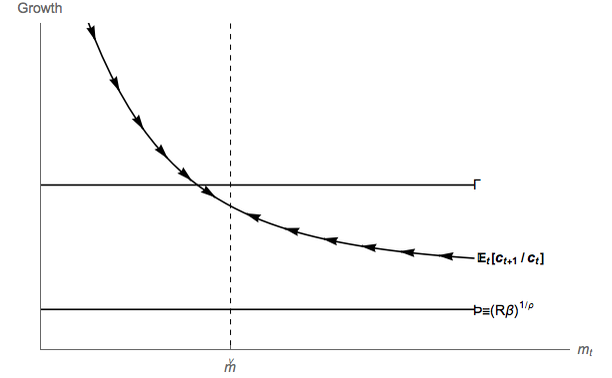
\includegraphics[width=6in]{\FigDir/cGroTargetFig}}
\caption{Target $\mRat$, Expected Consumption Growth, and Permanent Income Growth}
\label{fig:cGroTargetFig}
\end{figure}

\hypertarget{LimitsAsmtToInfty}{}
\subsection{Limits as $\mRat_t \uparrow \infty$}

\label{subsec:LimitsAsmtToInfty}

Define
\begin{eqnarray}
   \ushort{\cFunc}(\mRat) & = & \MinMPC \mRat \nonumber
\end{eqnarray}
which is the solution to an infinite-horizon problem with no noncapital
income
($\tShkAll_{t+n} = 0~\forall~n\geq1$); 
  clearly $\ushort{\cFunc}(\mRat)
< \cFunc(\mRat)$, since allowing the possibility of future noncapital
income cannot reduce current consumption.\footnote{We will assume the
  RIC holds here and subsequently so that $\MinMPC > 0$; the situation
  is a bit more complex when the RIC does not hold.   In that case the bound on consumption is given by the spending
  that would be undertaken by a consumer who faced binding liquidity
  constraints.  Detailed analysis of this special case is not
  sufficiently interesting to warrant inclusion in the paper.}

Assuming the FHWC holds, the infinite horizon perfect
foresight solution \eqref{eq:cFuncPFUnc} constitutes an upper
bound on consumption in the presence of uncertainty, since Carroll and
Kimball~\citeyearpar{ckConcavity} show that the introduction of
uncertainty strictly decreases the level of consumption at any $\mRat$.

Thus, we can write
\begin{eqnarray}  \label{eq:lowerltupper}
\ushort{\cFunc}(\mRat) < & \cFunc(\mRat) & < \bar{\cFunc}(\mRat) \nonumber \\
1 < & \cFunc(\mRat)/\ushort{\cFunc}(\mRat) & < \bar{\cFunc}(\mRat)/\ushort{\cFunc}(\mRat). \nonumber
\end{eqnarray}
But
\begin{eqnarray}  \label{eq:limitlowerupper}
\lim_{m \uparrow \infty} \bar{\cFunc}(\mRat)/\ushort{\cFunc}(\mRat) & = &
\lim_{m \uparrow \infty} (\mRat -1+ \hRat)/\mRat \nonumber \\
& = & 1, \nonumber
\end{eqnarray}
so as $\mRat \uparrow \infty, \cFunc(\mRat)/\ushort{\cFunc}(\mRat)
\rightarrow 1$, and the continuous differentiability and strict
concavity of $\cFunc(\mRat)$ therefore implies
\begin{equation}  \label{eq:limxtoinftycp}
\lim_{m \uparrow \infty} \cFunc^{\prime}(\mRat) =
\ushort{\cFunc}^{\prime}(\mRat) = \bar{\cFunc}^{\prime}(\mRat) = \MinMPC \notag
\end{equation}
because any other fixed limit would eventually lead to a level of
consumption either exceeding $\bar{\cFunc}(\mRat)$ or lower than
$\ushort{\cFunc}(\mRat)$.

Figure~\ref{fig:mpclimits} confirms these limits visually.  The top
plot shows the converged consumption function along with its upper and lower bounds,
while the lower plot shows the marginal propensity to consume.
\renewcommand{\figFile}{MPCLimits}
\hypertarget{\figFile}{}
\begin{figure}
\centerline{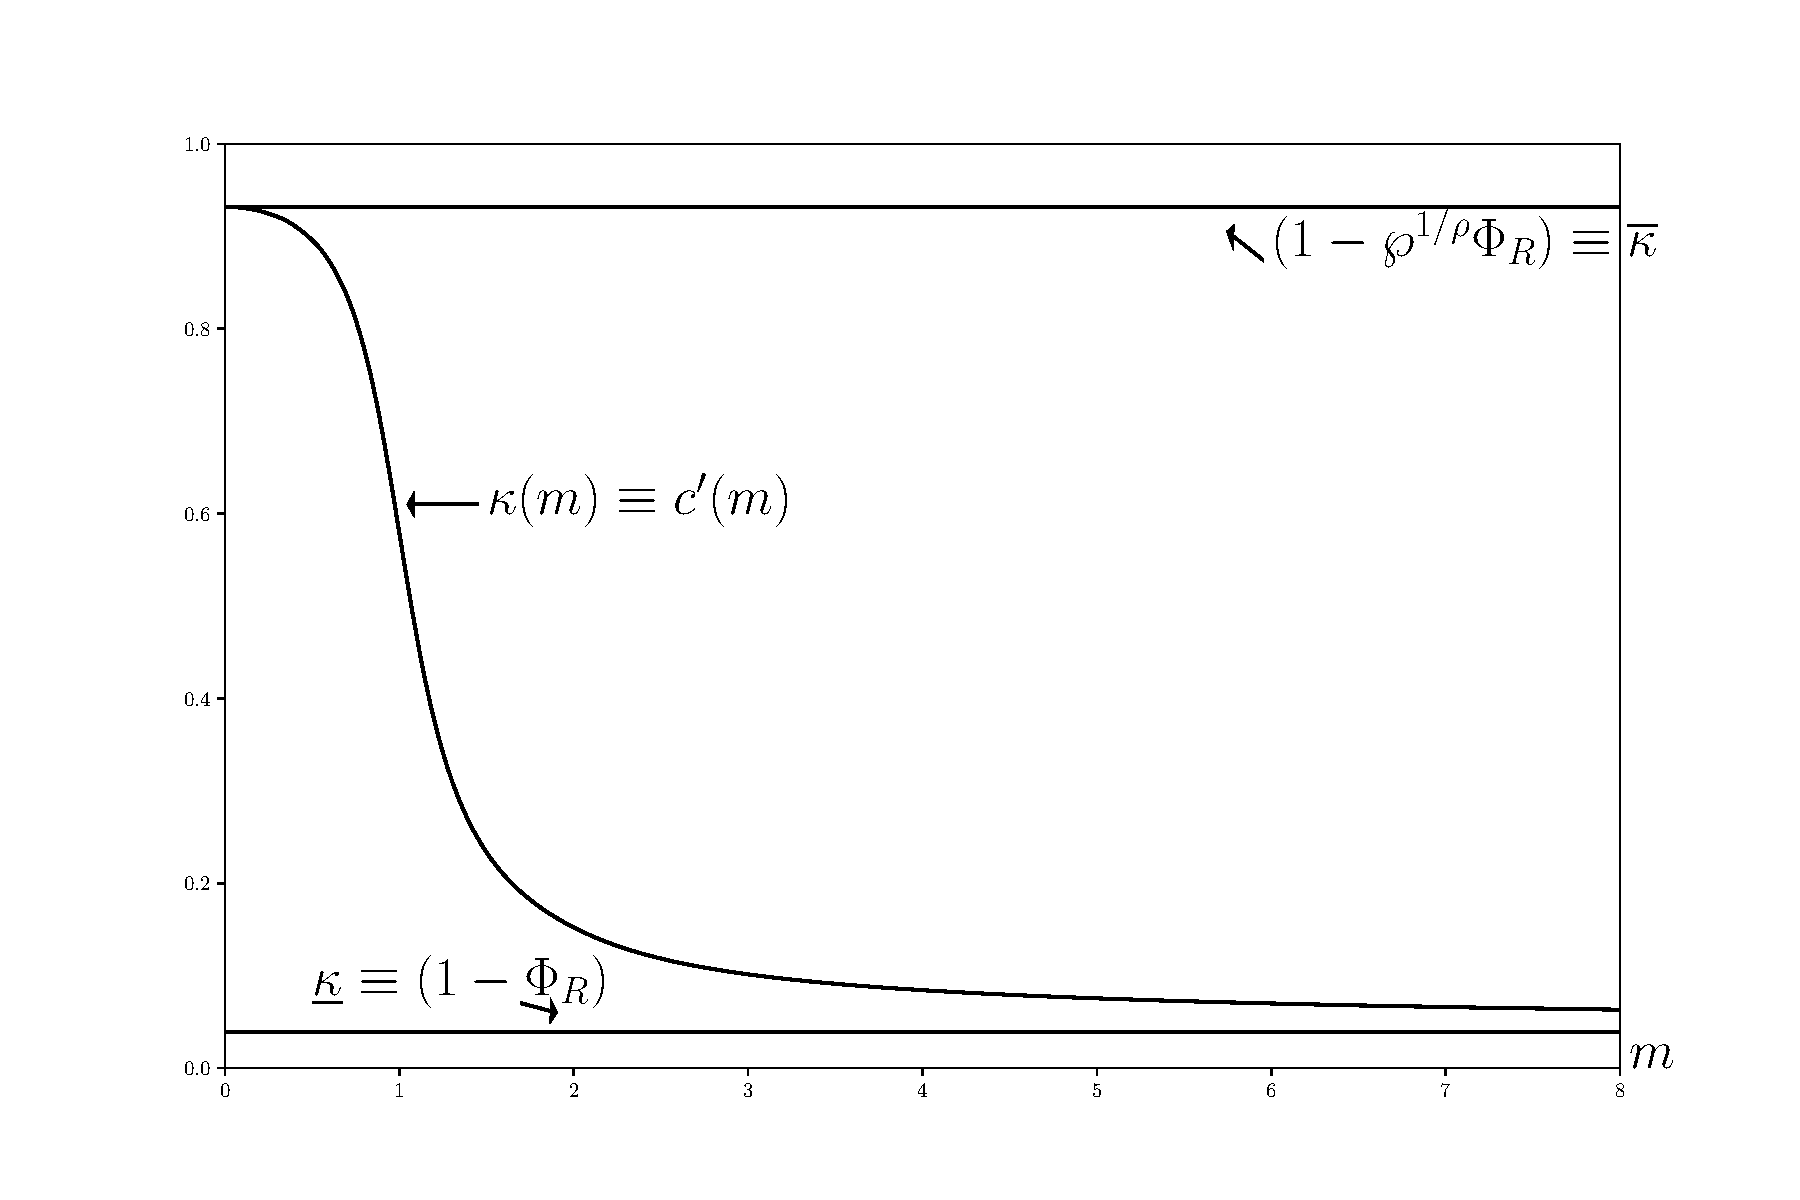
\includegraphics[width=6in]{\FigDir/MPCLimits}}
\caption{Limiting MPC's}
\label{fig:mpclimits}
\end{figure}

\renewcommand{\figFile}{cFuncBounds}
\hypertarget{\figFile}{}
\begin{figure}
\centering
\subfigure[\large Bounds]{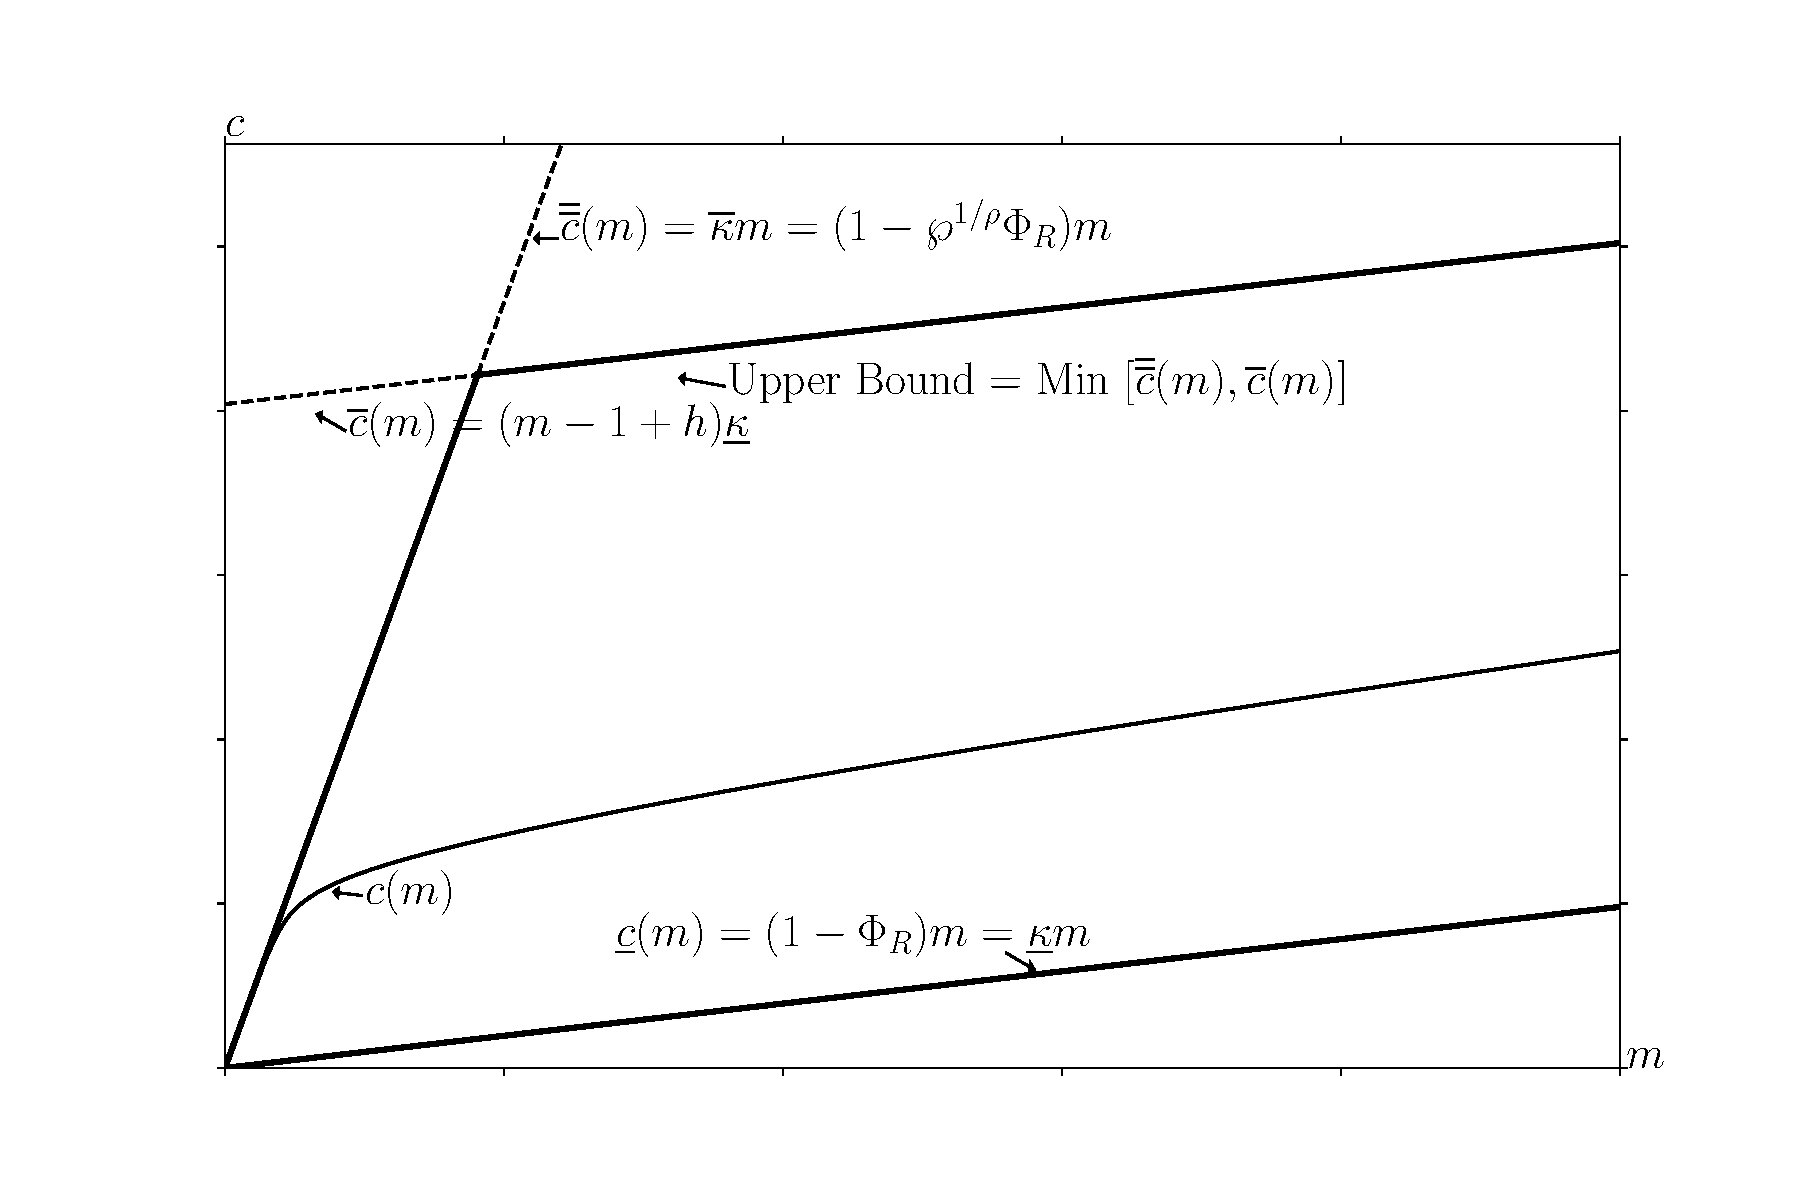
\includegraphics[width=6in]{\FigDir/cFuncBounds}}
\subfigure[\large Target $\mRat$]{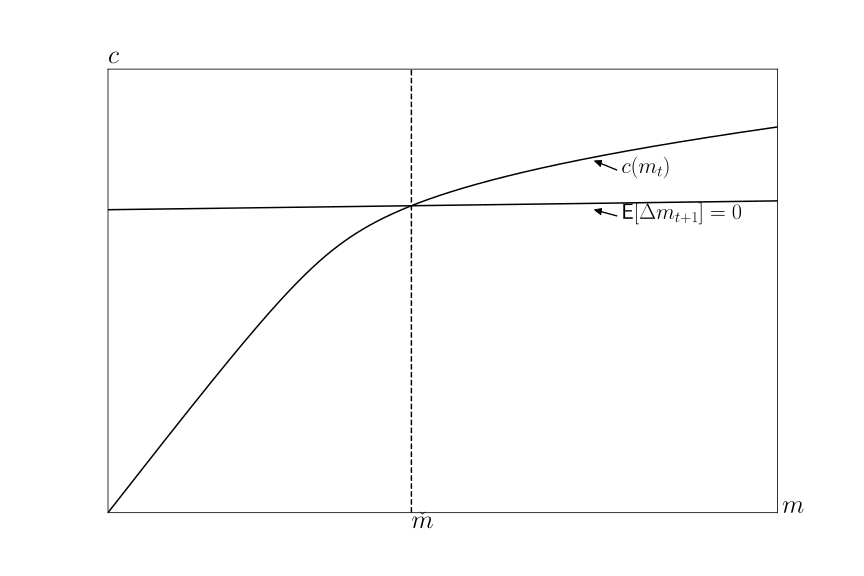
\includegraphics[width=6in]{\FigDir/cRatTargetFig}}
\caption{The Consumption Function}
\label{fig:cFuncBounds}
\end{figure}

Next we establish the limit of the expected consumption growth factor
as $\mRat_{t} \uparrow \infty$:
\begin{eqnarray}
\lim_{\mRat_{t} \uparrow \infty} \Ex_{t}[
\cLevBF_{t+1}/\cLevBF_{t}] & = & \lim_{\mRat_{t} \uparrow \infty} \Ex_{t}[
{\PGro}_{t+1} {\cRat}_{t+1}/c_{t}]. \notag
\end{eqnarray}

But
\begin{eqnarray*}
\Ex_{t}[{\PGro}_{t+1} {\ushort{\cRat}}_{t+1}/\bar{\cRat_{t}}] \leq \Ex_{t}[{\PGro}_{t+1} {\cRat}_{t+1}/\cRat_{t}] \leq \Ex_{t}[{\PGro}_{t+1} {\bar{\cRat}}_{t+1}/\ushort{\cRat}_{t}]
\end{eqnarray*}
and
\begin{equation}  \label{eq:xttoinfty}
\lim_{\mRat_t \uparrow \infty} \PGro_{t+1}\ushort{\cFunc}(\mRat_{t+1})/\bar{\cFunc}(\mRat_t) =
\lim_{\mRat_{t} \uparrow \infty} \PGro_{t+1}\bar{\cFunc}(\mRat_{t+1})/\ushort{\cFunc}(\mRat_t) =
\lim_{\mRat_{t} \uparrow \infty}\PGro_{t+1} \mRat_{t+1}/\mRat_t,  \notag
\end{equation}
while
\begin{eqnarray*}  \label{eq:xtp1toinfty}
\lim_{m_{t} \uparrow \infty} \PGro_{t+1} \mRat_{t+1}/\mRat_t & = & \lim_{m_{t} \uparrow \infty}
\left(\frac{\Rfree \aFunc(\mRat_t)+{\PGro}_{t+1}\tShkAll_{t+1}}{\mRat_t}\right)
\\ & = & (\Rfree \DiscFac)^{1/\CRRA} = \Pat
\end{eqnarray*}
because $\lim_{\mRat_{t}\uparrow \infty} \aFunc^{\prime}(\mRat)=\PatR$\footnote{This is because $\lim_{\mRat_{t}\uparrow \infty} \aFunc(\mRat_{t})/\mRat_{t}=1-\lim_{\mRat_{t}\uparrow \infty} \cFunc(\mRat_{t})/\mRat_{t}=1-\lim_{\mRat_{t}\uparrow \infty}\cFunc^{\prime}(\mRat_{t})=\PatR$.} and
$\PGro_{t+1}\tShkAll_{t+1}/\mRat_{t} \leq (\PGro \bar{\pShk} \bar{\tShkEmp}/\pNotZero )/\mRat_{t}$ which
goes to zero as $\mRat_{t}$ goes to infinity.

Hence we have
\begin{equation}
  {\Pat}  \leq \lim_{\mRat_{t} \uparrow \infty} \Ex_{t}[\cLevBF_{t+1}/\cLevBF_{t}] \leq {\Pat} \nonumber
\end{equation}
so as cash goes to infinity, consumption growth approaches its
value $\Pat$ in the perfect foresight model.

This argument applies equally well to the problem of the restrained
consumer, because as $\mRat$ approaches infinity the constraint becomes
irrelevant (assuming the FHWC holds).

\begin{comment}
Of course, the constraint never becomes irrelevant if human wealth is
infinite.  We ruled out infinite human wealth at the beginning of this
section by assuming $\Rfree> \PGro$.  If this finite human wealth
condition does not hold, it is possible to show that for any finite
horizon consumer the marginal propensity to consume approaches the
finite-horizon perfect foresight MPC as wealth approaches infinity.
However, as the horizon gets longer, the perfect foresight MPC
approaches zero.  It can be shown therefore that the limiting MPC for
the converged consumption function approaches (but never reaches)
zero.  (This is why we chose $\MinMinMPC=0$ if the FHWC fails
in the proofs above.)
\end{comment}

\hypertarget{LimitsAsmtToZero}{}
\subsection{Limits as $\mRat_t \downarrow 0$}

\label{subsec:LimitsAsmtToZero} Now consider the limits of behavior as $\mRat_{t}$ gets
arbitrarily small.

Equation \eqref{eq:MaxMPCDef} shows that the limiting value of
$\MaxMPC$ is
\begin{eqnarray}
 \MaxMPC & = & 1-{\Rfree}^{-1}(\pZero  \Rfree\DiscFac)^{1/\CRRA}. \nonumber
\end{eqnarray}

Defining $\eFunc(\mRat)=\cFunc(\mRat)/\mRat$ as before we have
\begin{eqnarray}
  \lim_{m \downarrow 0} \eFunc(\mRat) & = & (1-\pZero^{1/\CRRA}\PatR) = \MaxMPC \nonumber.
\end{eqnarray}

Now using the continuous differentiability of the consumption function
along with L'H\^opital's rule, we have
\begin{comment}
\begin{eqnarray*}
    \eFunc^{\prime}(\mRat) & = & \mRat^{-1} \cFunc^{\prime}(\mRat) - \mRat^{-2} \cFunc(\mRat)
\\ \mRat \eFunc^{\prime}(\mRat) & = & \cFunc^{\prime}(\mRat) - \cFunc(\mRat)/\mRat
\\ \cFunc^{\prime}(\mRat) & = & \eFunc(\mRat)+ \mRat \eFunc^{\prime}(\mRat)
\end{eqnarray*}
and since $0<\eFunc(\mRat)<1$ we have
\end{comment}
\begin{eqnarray}
  \lim_{m \downarrow 0} \cFunc^{\prime}(\mRat) & = & \lim_{m \downarrow 0}
  \eFunc(\mRat) = \MaxMPC. \nonumber
\end{eqnarray}

Figure~\ref{fig:mpclimits} confirms that the numerical solution method
obtains this limit for the MPC as $\mRat$ approaches zero.

For consumption growth, as $\mRat \downarrow 0$ we have
\begin{eqnarray*}
\lim_{\mRat_{t} \downarrow 0} \Ex_{t}\left[\left(\frac{\cFunc({\mRat}_{t+1})}{\cFunc(\mRat_t)}\right){\PGro}_{t+1}\right]
& > & \lim_{\mRat_{t} \downarrow 0} \Ex_{t}\left[\left(\frac{\ushort{\cFunc}({\mathcal{\mathcal{R}}}_{t+1}\aFunc(\mRat_{t})+{%
\tShkAll}_{t+1})}{\MaxMPC \mRat_{t}}\right){\PGro}_{t+1}\right]  \notag \\
& = & \phantom{+}\pZero \lim_{\mRat_{t} \downarrow 0} \Ex_{t}\left[\left(\frac{\ushort{\cFunc}({\mathcal{\mathcal{R}}}_{t+1}\aFunc(\mRat_{t}))}{\MaxMPC \mRat_{t}}\right){\PGro}_{t+1}\right] \\
& & + \pNotZero \lim_{\mRat_{t} \downarrow 0}  \Ex_{t}\left[\left(\frac{\ushort{\cFunc}({\mathcal{\mathcal{R}}}_{t+1}\aFunc(\mRat_{t})+
\tShkEmp_{t+1}/\pNotZero)}{\MaxMPC \mRat_{t}}\right){\PGro}_{t+1}\right]  \\\notag
& > & \pNotZero \lim_{\mRat_{t} \downarrow 0} \Ex_{t}\left[\left(\frac{\ushort{\cFunc}(
\tShkEmp_{t+1}/\pNotZero)}{\MaxMPC \mRat_{t}}\right){\PGro}_{t+1}\right] \\
& = & \infty \nonumber
\end{eqnarray*}
where the second-to-last line follows because  $\lim_{\mRat_{t} \downarrow 0} \Ex_{t}\left[\left(\frac{\ushort{\cFunc}({\mathcal{\mathcal{R}}}_{t+1}\aFunc(\mRat_{t}))}{\MaxMPC \mRat_{t}}\right){\PGro}_{t+1}\right]$ is positive, and the last line follows because the minimum possible realization of $\tShkEmp_{t+1}$ is $\ushort{\tShkEmp}>0$ so the minimum possible value of expected next-period consumption is positive.\footnote{
The same arguments establish $\lim_{m \downarrow 0} \Ex_{t}[\cLevBF_{t+1}/\cLevBF_{t}] = \infty$
for the problem of the restrained consumer.%
}

\hypertarget{onetarget}{}
\subsection{There Exists Exactly One Target Cash-on-Hand Ratio,
which is Stable}

\label{subsec:onetarget}

Define the target cash-on-hand-to-income ratio $\mTarg$ as the value of $\mRat$
such that
\begin{equation}  \label{eq:mTarget}
\Ex_t [{\mRat}_{t+1}/\mRat_t] = 1 \mbox{~if~} \mRat_t = \mTarg.
\end{equation}
where the $\vee$ accent is meant to invoke the fact that this is the value that other $\mRat$'s `point to.'

We prove existence by arguing that $\Ex_t [{\mRat}_{t+1}/\mRat_t]$ is
continuous on $\mRat_{t}>0$, %
and takes on values both above and below 1,
so that it must equal 1 somewhere by the intermediate
value theorem.

Specifically, the same logic used in section~\ref{subsec:LimitsAsmtToZero} shows
that $\lim_{\mRat_t \downarrow 0} \Ex_t [{\mRat}_{t+1}/\mRat_t] =
\infty$.

The limit as $\mRat_{t}$ goes to infinity is
\begin{eqnarray*}
  \lim_{\mRat_{t} \uparrow \infty} \Ex_{t}[{\mRat}_{t+1}/\mRat_{t}] & = &   \lim_{\mRat_{t} \uparrow \infty} \Ex_{t}\left[\frac{{\mathcal{\mathcal{R}}}_{t+1}\aFunc(\mRat_{t})+{\tShkAll}_{t+1}}{\mRat_{t}}\right]
\\ & = & \Ex_{t}[(\Rfree/{\PGro}_{t+1})\PatR]
\\ & = & \Ex_{t}[{\Pat}/{\PGro}_{t+1}]
\\ & < & 1
\end{eqnarray*}
where the last line is guaranteed by our imposition of the GIC \eqref{eq:GIC}.

Stability means that in a local neighborhood of $\mTarg$, values of $\mRat_{t}$
above $\mTarg$ will result in a smaller ratio of $\Ex_{t}[{\mRat}%
_{t+1}/\mRat_{t}] $ than at $\mTarg$. That is, if $\mRat_{t} > \mTarg$ then $%
\Ex_{t}[\mRat_{t+1}/\mRat_{t}] < 1 $. This will be true if
\begin{eqnarray}
\left(\frac{d}{d\mRat_t}\right) \Ex_t [{\mRat}_{t+1}/\mRat_t ] & < & 0 \label{eq:stable} \nonumber
\end{eqnarray}
at $\mRat_{t}=\mTarg$.  But \providecommand{\numFunc}{\pmb{\zeta}}
\begin{eqnarray*}
\left( \frac{d}{d\mRat_{t}}\right) \Ex_{t}[{\mRat}_{t+1}/\mRat_{t}] &=&\Ex_{t}\left[
\left( \frac{d}{d\mRat_{t}}\right) \left[ {\Rnorm}_{t+1}(1-\cFunc(\mRat_{t})/\mRat_{t})+%
{\tShkAll}_{t+1}/\mRat_{t}\right] \right]  \nonumber \\
&=&\Ex_{t}\left[ \frac{{\Rnorm}_{t+1}(\cFunc(\mRat_{t})-\cFunc^{\prime}(\mRat_{t})\mRat_{t})-%
{\tShkAll}_{t+1}}{\mRat_{t}^{2}}\right]  \notag
\end{eqnarray*}
which will be negative if its numerator is negative. Define $\numFunc(\mRat_{t})$
as the expectation of the numerator,
\begin{equation}
\numFunc (\mRat_{t})=\underbrace{\Ex_{t}[{\Rnorm}_{t+1}]}_{\equiv \bar{\Rnorm}}(\cFunc(\mRat_{t})-\cFunc^{\prime}(\mRat_{t})\mRat_{t})-1. \label{eq:numer}
\end{equation}

The target level of market resources is the $\mRat$ such that if $\mRat_{t}=\mTarg$ then $\Ex_{t}[\mRat_{t+1}]=\mTarg$.
\begin{eqnarray}
\Ex_{t}[{\mRat}_{t+1}] & = & \Ex_{t}[{\Rnorm}_{t+1}(\mRat_{t}-c_{t})+{%
\tShkAll}_{t+1}] \nonumber \\
\mTarg & = & \bar{\Rnorm}(\mTarg-\cFunc(\mTarg))+1  \nonumber \\
\bar{\Rnorm}\cFunc(\mTarg) & = & 1+(\bar{\Rnorm}-1)\mTarg  \label{eq:cstar}.
\end{eqnarray}

At the target, equation \eqref{eq:numer} is
\begin{eqnarray}
\numFunc(\mTarg) & = & \bar{\Rnorm}\cFunc(\mTarg) - \bar{\Rnorm}\cFunc^{\prime}(\mTarg)\mTarg - 1.  \label{eq:numerxstar} \nonumber
\end{eqnarray}

Substituting for the first term in this expression using
\eqref{eq:cstar} gives
\begin{eqnarray*}
\numFunc(\mTarg) & = & 1+(\bar{\Rnorm}-1)\mTarg- \bar{\Rnorm}\cFunc^{\prime}(\mTarg)\mTarg - 1 \\
& = & \mTarg\left(\bar{\Rnorm}-1-\bar{\Rnorm}\cFunc^{\prime}(\mTarg)\right) \\
& = & \mTarg\left(\bar{\Rnorm}(1-\cFunc^{\prime}(\mTarg))-1\right) \\
& < & \mTarg\left(\bar{\Rnorm}(1-(1-{\Rfree}^{-1}(\Rfree\DiscFac)^{1/%
\CRRA}))-1\right) \\
& = & \mTarg\left(\bar{\Rnorm}\PatR-1%
\right) \\
& = & \mTarg\left(\underbrace{\Ex_{t}[{\Pat}/{\PGro}_{t+1}]}_{<
1\text{~from \eqref{eq:GIC}}}-1\right) \\
& < & 0
\end{eqnarray*}
where the step introducing the inequality imposes the fact that $\cFunc^{\prime} > \PatR$ which is an
implication of the concavity of the consumption function.

We have now proven that some target $\mTarg$ must exist, and that at any such
$\mTarg$ the solution is stable. Nothing so far, however, rules
out the possibility that there will be multiple values of $\mRat$ that
satisfy the definition \eqref{eq:mTarget} of a target.

Multiple targets can be ruled out as follows. Suppose there exist
multiple targets; these can be arranged in ascending order and indexed
by an integer superscript, so that the target with the smallest value is,
e.g., $\mTarg^{1}$. The argument just completed implies that since
$\Ex_{t}[{\mRat}_{t+1}/\mRat_{t}]$ is continuously differentiable
there must exist some small $\epsilon$ such that
$\Ex_{t}[{\mRat}_{t+1}/\mRat_{t}] < 1$ for $\mRat_{t} =
\mTarg^{1}+\epsilon$. (Continuous differentiability of
$\Ex_{t}[{\mRat}_{t+1}/\mRat_{t}]$ follows from the continuous
differentiability of $\cFunc(\mRat_{t})$.) 

Now assume there exists a second value of $\mRat$ satisfying the
definition of a target, $\mTarg^{2}$. Since
$\Ex_{t}[{\mRat}_{t+1}/\mRat_{t}]$ is continuous, it must be
approaching 1 from below as $\mRat_{t} \rightarrow \mTarg^{2}$, since
by the intermediate value theorem it could not have gone above 1
between $\mTarg^{1}+\epsilon$ and $\mTarg^{2}$ without passing through
1, and by the definition of $\mTarg^{2}$ it cannot have passed through
1 before reaching $\mTarg^{2}$.  But saying that
$\Ex_{t}[{\mRat}_{t+1}/\mRat_{t}]$ is approaching 1 from below as
$\mRat_{t} \rightarrow \mTarg^{2}$ implies that
\begin{eqnarray}
\left(\frac{d}{d\mRat_{t}}\right)\Ex_{t}[{\mRat}_{t+1}/\mRat_{t}] & > & 0
\label{eq:badeqn}
\end{eqnarray}
at $\mRat_{t}=\mTarg^{2}$. However, we just showed above that, under
our assumption that the GIC holds, precisely the opposite of equation
\eqref{eq:badeqn} must hold for any $\mRat$ that satisfies the definition
of a target. Thus, assuming the existence of more than one target
implies a contradiction.

The foregoing arguments rely on the continuous differentiability of
$\cFunc(\mRat)$, so the arguments do not directly go through for the
restrained consumer's problem in which the existence of liquidity
constraints can lead to discrete changes in the slope
$\cFunc^{\prime}(\mRat)$ at particular values of $\mRat$. But we can
use the fact that the restrained model is the limit of the baseline
model as $\pZero \downarrow 0$ to conclude that there is likely a
unique target cash level even in the restrained model.

If consumers are sufficiently impatient, the limiting target level in the
restrained model will be $\mTarg = \Ex_{t}[{\tShkAll}_{t+1}] = 1$. That
is, if a consumer starting with $\mRat = 1$ will save nothing, ${\aFunc}(1)=0$,
then the target level of $\mRat$ in the restrained model will be 1; if a
consumer with $\mRat=1$ would choose to save something, then the target
level of cash-on-hand will be greater than the expected level of income.

\hypertarget{cGroLTpGro}{}
\subsection{Expected Consumption Growth at Target $\mRat$ Is Less than
Expected Permanent Income Growth}

\label{subsec:expcgrowth} In Figure~\ref{fig:cGroTargetFig} the intersection of
the target cash-on-hand ratio locus at $\mTarg$ with the expected consumption
growth curve lies below the intersection with the horizontal line
representing the growth rate of expected permanent income. This can be
proven as follows.

Strict concavity of the consumption function implies that if $\Ex_{t}[{\mRat}%
_{t+1}] = \mTarg = \mRat_{t}$ then
\begin{eqnarray}
\Ex_{t}\left[\frac{{\PGro}_{t+1} \cFunc({\mRat}_{t+1})}{\cFunc(\mRat_{t})}
\right] & < & \Ex_{t}\left[\left(\frac{{\PGro}_{t+1}
(\cFunc(\mTarg)+\cFunc^{\prime}(\mTarg)({\mRat}_{t+1}-\mTarg))}{\cFunc(\mTarg)}\right)\right]  \nonumber
\\
& = & \Ex_{t}\left[{\PGro}_{t+1} \left(1+\left(\frac{\cFunc^{\prime}(\mTarg)}{%
\cFunc(\mTarg)}\right)({\mRat}_{t+1}-\mTarg)\right)\right]  \nonumber  \\
& = & \PGro + \left(\frac{\cFunc^{\prime}(\mTarg)}{\cFunc(\mTarg)}\right)\Ex_{t}\left[ {\PGro}_{t+1}\left({\mRat}_{t+1}-\mTarg\right)\right]  \nonumber \\
& = & \PGro + \left(\frac{\cFunc^{\prime}(\mTarg)}{\cFunc(\mTarg)}\right)\left[
\Ex_{t}[ \PGro_{t+1}]\underbrace{\Ex_{t}[
{\mRat}_{t+1}-\mTarg]}_{=0}+\mbox{cov}_{t}( {\PGro}_{t+1},{\mRat}_{t+1})\right]
 \label{eq:covcgrow}
\end{eqnarray}
and since $\mRat_{t+1} = (\Rfree/\PGro_{t+1}) \aFunc(\mTarg)+\tShkAll_{t+1}$ and
$\aFunc(\mTarg)>0$ it is clear that
cov$_{t}({\PGro}_{t+1},{\mRat}_{t+1})<0$ which implies that
the entire term added to $\PGro$ in \eqref{eq:covcgrow} is negative, as
required.

\hypertarget{dcgdxneg}{}
\subsection{Expected Consumption Growth Is a Declining Function of $\mRat_{t}$ (or Is It?)}
\label{subsec:dcgdxneg}

Figure~\ref{fig:cGroTargetFig} depicts the expected consumption growth factor as a strictly
declining function of the cash-on-hand ratio. To investigate this,
define
\begin{eqnarray*}
\pmb{\Upsilon}(\mRat_{t}) & \equiv & \PGro_{t+1} \cFunc(\Rnorm_{t+1}\aFunc(\mRat_{t})+\tShkAll_{t+1})/\cFunc(\mRat_{t})  = \cLevBF_{t+1}/\cLevBF_{t}
\end{eqnarray*}
and the proposition in which we are interested is

\begin{eqnarray}
  (d/d\mRat_{t})\Ex_{t}[\underbrace{\pmb{\Upsilon}(\mRat_{t})}_{\equiv \pmb{\Upsilon}_{t+1}}] & < & 0 \label{eq:dChi}  \nonumber
\end{eqnarray}
or differentiating through the expectations operator, what we want is
\begin{eqnarray}
\Ex_{t}\left[\PGro_{t+1} \left(\frac{\cFunc^{\prime}(\mRat_{t+1})\Rnorm_{t+1}\aFunc^{\prime}(\mRat_{t})\cFunc(\mRat_{t})-\cFunc(\mRat_{t+1})\cFunc^{\prime}(\mRat_{t})}{\cFunc(\mRat_{t})^{2}}\right)\right] & < & 0 \label{eq:kappaPrimeLT0}.
\end{eqnarray}

Henceforth indicating appropriate arguments by the corresponding
subscript (e.g.\ $\cFunc_{t+1}^{\prime} \equiv \cFunc^{\prime}(\mRat_{t+1})$), since
$\PGro_{t+1}\Rnorm_{t+1}=\Rfree$, the portion of the LHS of equation \eqref{eq:kappaPrimeLT0} in brackets can be manipulated to yield
\begin{eqnarray}
 \cFunc_{t} \pmb{\Upsilon}^{\prime}_{t+1} & = & \cFunc^{\prime}_{t+1}\aFunc^{\prime}_{t}\Rfree-\cFunc^{\prime}_{t} \PGro_{t+1} \cFunc_{t+1}/\cFunc_{t} \nonumber
\\ & = & \cFunc^{\prime}_{t+1}\aFunc^{\prime}_{t}\Rfree-\cFunc^{\prime}_{t} \pmb{\Upsilon}_{t+1} \label{eq:cPrimek}
.
\end{eqnarray}

Now differentiate the Euler equation with respect to $\mRat_{t}$:
\begin{eqnarray}
  1 & = & \Rfree \DiscFac \Ex_{t}[ \pmb{\Upsilon}_{t+1}^{-\CRRA}] \notag
\\ 0 & = & \Ex_{t}[\pmb{\Upsilon}_{t+1}^{-\CRRA-1} \pmb{\Upsilon}_{t+1}^{\prime}] \notag
\\ & = & \Ex_{t}[\pmb{\Upsilon}_{t+1}^{-\CRRA-1}]\Ex_{t}[\pmb{\Upsilon}_{t+1}^{\prime}]+\mbox{cov}_{t}(\pmb{\Upsilon}_{t+1}^{-\CRRA-1},\pmb{\Upsilon}_{t+1}^{\prime}) \notag
\\ \Ex_{t}[\pmb{\Upsilon}_{t+1}^{\prime}] & = & -\mbox{cov}_{t}(\pmb{\Upsilon}_{t+1}^{-\CRRA-1},\pmb{\Upsilon}_{t+1}^{\prime})/\Ex_{t}[\pmb{\Upsilon}_{t+1}^{-\CRRA-1}] \label{eq:covgen}
\end{eqnarray}
but since $\pmb{\Upsilon}_{t+1} > 0$ we can see from \eqref{eq:covgen} that \eqref{eq:kappaPrimeLT0} is equivalent to
\begin{eqnarray}
 \mbox{cov}_{t}(\pmb{\Upsilon}_{t+1}^{-\CRRA-1},\pmb{\Upsilon}_{t+1}^{\prime}) & > & 0 \nonumber
\end{eqnarray}
which, using \eqref{eq:cPrimek}, will be true if
\begin{eqnarray}
 \mbox{cov}_{t}(\pmb{\Upsilon}_{t+1}^{-\CRRA-1},\cFunc^{\prime}_{t+1}\aFunc^{\prime}_{t}\Rfree - \cFunc^{\prime}_{t}\pmb{\Upsilon}_{t+1}) & > & 0 \notag
\end{eqnarray}
which in turn will be true if both
\begin{eqnarray}
  \mbox{cov}_{t}(\pmb{\Upsilon}_{t+1}^{-\CRRA-1},\cFunc^{\prime}_{t+1} ) & > & 0 \notag
\end{eqnarray}
and
\begin{eqnarray*}
  \mbox{cov}_{t}(\pmb{\Upsilon}_{t+1}^{-\CRRA-1},\pmb{\Upsilon}_{t+1}) & < & 0. \notag
\end{eqnarray*}

The latter proposition is obviously true under our assumption $\CRRA > 1$.  The former will be true if
\begin{eqnarray*}
  \mbox{cov}_{t}\left((\PGro \pShk_{t+1} \cFunc(\mRat_{t+1}))^{-\CRRA-1},\cFunc^{\prime}(\mRat_{t+1}) \right) & > & 0 \nonumber.
\end{eqnarray*}}

The two shocks cause two kinds of variation in $\mRat_{t+1}$.
Variations due to $\tShkAll_{t+1}$ satisfy the proposition, since a
higher draw of $\tShkAll$ both reduces $c_{t+1}^{-\CRRA-1}$ and
reduces the marginal propensity to consume.  However, permanent shocks
have conflicting effects.  On the one hand, a higher draw of
$\pShk_{t+1}$ will reduce $\mRat_{t+1}$, thus increasing both
$c_{t+1}^{-\CRRA-1}$ and $c_{t+1}^{\prime}$.  On the other hand, the
$c_{t+1}^{-\CRRA-1}$ term is multiplied by $\PGro \pShk_{t+1}$, so the
effect of a higher $\pShk_{t+1}$ could be to decrease the first term
in the covariance, leading to a negative covariance with the second
term.  (Analogously, a lower permanent shock $\pShk_{t+1}$ can also
lead a negative correlation.)

The software archive associated with this paper presents an example in
which this perverse effect dominates.  However, extreme assumptions
were required (in particular, a very small probability of the
zero-income shock) and the region in which
$\pmb{\Upsilon}_{t+1}^{\prime} > 0$ was tiny.  In practice, for
plausible parametric choices,
$\Ex_{t}[\pmb{\Upsilon}_{t+1}^{\prime}]<0$ should generally hold.

\hypertarget{The-Aggregate-and-Idiosyncratic-Relationship-Between-Consumption-Growth-and-Income-Growth}{}
\section{The Aggregate and Idiosyncratic Relationship Between
Consumption Growth and Income Growth}

This section examines the behavior of large collections of buffer-stock consumers with identical parameter values. Such a collection can be thought of as either a subset of the population within a single country (say, members of a given education or occupation group), or as the whole population in a small open economy.\footnote{We will continue to take the aggregate interest rate as exogenous and constant. It is also possible, and only slightly more difficult, to solve for the steady-state of a closed-economy version of the model where the interest rate is endogenous.}

Formally, we assume a continuum of {\it ex ante} identical households
on the unit interval, with constant total mass normalized to one and
indexed by $i \in [0,1]$, all behaving according to the model
specified above.\footnote{One inconvenient aspect of the model as
  specified is that it does not exhibit a stationary distribution of
  idiosyncratic permanent noncapital income; the longer the economy lasts, the wider is the
  distribution.  This problem can be remedied by assuming a constant
  probability of death, and replacing deceased households with
  newborns whose initial idiosyncratic permanent income matches the
  mean idiosyncratic permanent income of the population.  For a fully
  worked-out general equilibrium version of such a model, see \cite{BSinKS}.}

Szeidl~\citeyearpar{szeidlInvariant} proves that such a
population will be characterized by an invariant
distribution of $\mRat$ that induces invariant distributions for $\cRat$ and
$\aRat$; designate these $\mathcal{F}^{\mRat}$, $\mathcal{F}^{\aRat}$, and
$\mathcal{F}^{\cRat}$.\footnote{Szeidl's proof supplants simulation evidence of ergodicity
that appeared in an earlier version of this paper.}

\begin{comment}
  \hypertarget{Convergence-of-the-Cross-Section-Distribution}{}
\subsection{Convergence of the Cross-Section Distribution}

Szeidl's proof, however, does not yield any sense of how quickly
convergence occurs, which in principle depends on all of the
parameters of the model as well as the initial conditions.  To build
intuition, Figure~\ref{fig:simcdfsconverge} supplies an example in
which a population begins with a particularly simple distribution that
is far from the invariant one:
\begin{eqnarray*}
  \mRat_{1,i} & = & \tShkAll_{1,i},
\end{eqnarray*}
which would characterize a population in which all assets had been
wiped out immediately before the receipt of period 1's noncapital
income.\footnote{We assume that $\log\pShk_{t+1}$ and
  $\log\tShk_{t+1}$ are normally distributed with means
  $-\sigma^{2}_{\pshk}/2$ and $-\sigma^{2}_{\tshk}/2$ and variances
  $\sigma^{2}_{\pshk}$ and $\sigma^{2}_{\tshk}$ (so that
  $\Mean[\pShk_{t+1}]=\Mean[\tShk_{t+1}]=1$), where $\Mean[]$ is the mean operator defined below.}

The figure plots the
distributions of $\aRat$ (for technical reasons, this is slightly
better than plotting $\mRat$) at the ends of 1, 4, 10, and 40
periods.\footnote{The figure reflects results for the calibration
  detailed in Table 1, which are representative of the micro
  literature which has mainly focused on matching behavior of median
  or ``typical'' households, who hold little liquid wealth.  A higher
  time preference factor would be necessary to match the behavior of
  richer households who hold much of the aggregate capital stock.
  However, for these richer households, the precautionary motives
  highlighted in this model may be less relevant than other motives
  which are less well understood.}

\renewcommand{\figFile}{SimCDFsConverge}
\hypertarget{\figFile}{}
\begin{figure}[h]
\centerline{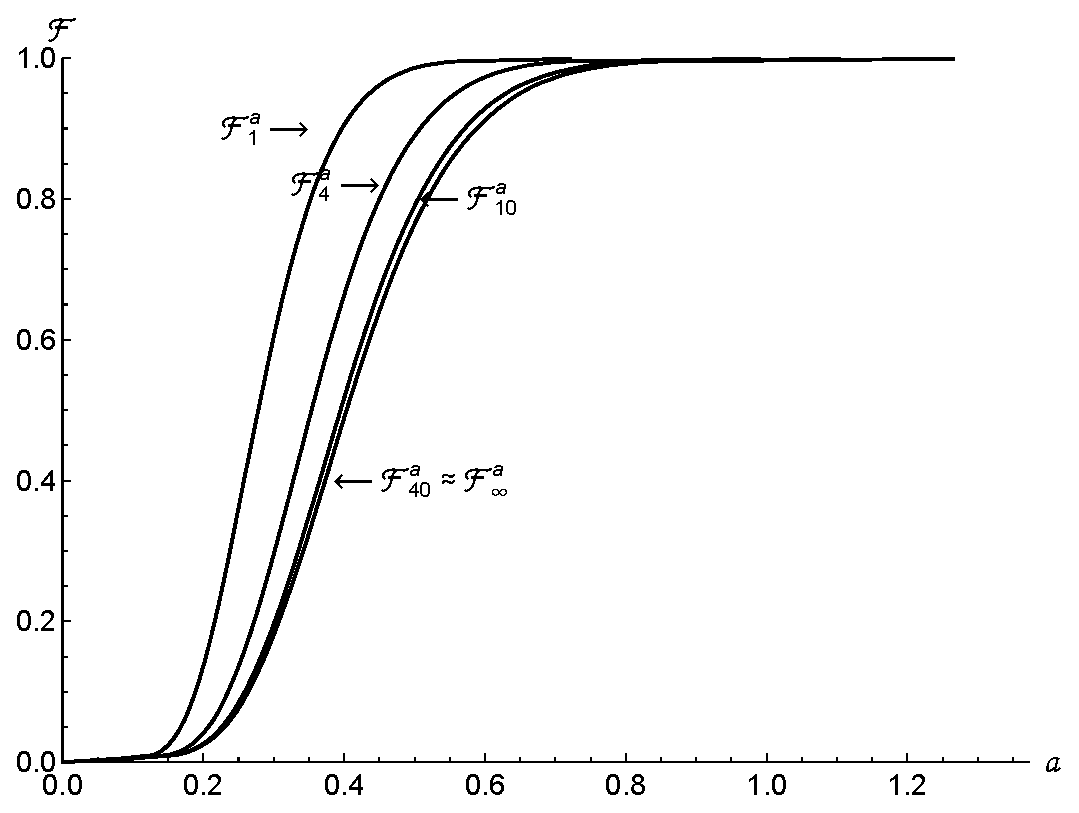
\includegraphics[width=6in]{\FigDir/SimCDFsConverge}}
\caption{Convergence of $\mathcal{F}^{\aRat}$ to Invariant Distribution}
\label{fig:simcdfsconverge}
\end{figure}


The figure illustrates the fact that, under these parameter values,
convergence to the invariant distribution has largely been
accomplished within 10 periods.  By 40 periods, the distribution is
indistinguishable from the invariant distribution.
\end{comment}

\hypertarget{Consumption-and-Income-Growth-at-the-Household-Level}{}
\subsection{Consumption and Income Growth at the Household Level}

It is useful to define the operator $\Mean\left[\bullet\right]$
which yields the mean value of its argument in the population, as
distinct from the expectations operator $\Ex\left[\bullet\right]$ which represents beliefs about the
future.

An economist with a microeconomic dataset could calculate the average
growth rate of idiosyncratic consumption, and would find
\begin{eqnarray*}
\Mean\left[\Delta \log \cLevBF_{t+1}\right] & = & \Mean\left[ \log {\cRat}%
_{t+1}\pLevBF_{t+1} - \log c_{t}\pLevBF_{t}\right]  \notag \\
& = & \Mean\left[ \log \pLevBF_{t+1}- \log \pLevBF_{t} + \log {\cRat}_{t+1} - \log c_{t}\right]  \notag \\
& = & \Mean\left[ \log \pLevBF_{t+1}- \log \pLevBF_{t}\right] + \Mean\left[ \log {\cRat}_{t+1} - \log c_{t}\right]  \notag \\
& = & (\gamma - \sigma^{2}_{\pshk}/2) + \Mean[\log \cRat_{t+1} - \log \cRat_{t}] \\
& = & (\gamma - \sigma^{2}_{\pshk}/2)
\end{eqnarray*}
where $\gamma=\log \PGro$ and the last equality follows because the invariance of
$\mathcal{F}^{\cRat}$ (see \cite{szeidlInvariant}) means that $\Mean\left[ \log
  {\cRat}_{t+n}\right] = \Mean\left[ \log
  c_{t}\right]$.\footnote{Papers in the simulation literature have
  observed an approximate equivalence between the average growth rates
  of idiosyncratic consumption and permanent income, but formal proof
  was not possible until Szeidl's proof of ergodicity.}

Thus, in a population that has reached its invariant distribution, the growth
rate of idiosyncratic log consumption matches the growth rate of idiosyncratic log permanent income.

\ShorterYN{}{
\hypertarget{Growth-Rates-of-Aggregate-Income-and-Consumption}{}
\subsection{Growth Rates of Aggregate Income and Consumption}
\label{subsec:cGroEqPGroQ}

Attanasio and Weber~\citeyearpar{aw95} point out that
concavity of the consumption function (or other nonlinearities) can
imply that it is quantitatively important to distinguish between the
growth rate of average consumption and the average growth rate of
consumption.\footnote{Since we assume number of the households are
  normalized to 1, aggregate and average variables are identical.}  We
have just examined the average growth rate; we now examine the growth
rate of the average.

Using capital letters for aggregate
variables, the growth factor for aggregate income is given by:
\begin{eqnarray*}
\YLevBF_{t+1}/\YLevBF_{t} & = & \Mean\left[\tShkAll_{t+1}\PGro \pShk_{t+1}\pLevBF_{t}\right]/\Mean\left[\pLevBF_{t}\tShkAll_{t}\right]
\\ & = & \PGro
\end{eqnarray*}
because of the independence assumptions we have made about $\tShkAll$ and $\pShk$.

Aggregate assets are:
\begin{eqnarray*}
\ALevBF_{t} &=&\Mean\left[ a_{t,i} \pLevBF_{t,i}\right]  \notag \\
&=& \ASS \PLevBF_{t}+\mbox{cov}_{t}(a_{t,i},\pLevBF_{t,i}) \label{eq:AAgg}
\end{eqnarray*}
where $\PLevBF_{t}$ designates the mean level of
permanent income across all individuals, and we are assuming that $\aRat_{t,i}$
was distributed according to the
invariant distribution with a mean value of $\ARat.$
Since permanent income grows at mean rate $\PGro$ while the
distribution of $\aRat$ is invariant, if we normalize $\PLevBF_{t}$ to one we
will similarly have for any period $n \geq 1$
\begin{eqnarray}
  \ALevBF_{t+n} & = & \ASS \PGro^{n} +\mbox{cov}(a_{t+n,i},\pLevBF_{t+n,i}). \notag
\end{eqnarray}

Unfortunately, \cite{szeidlInvariant}'s proof of the invariance of
$\mathcal{F}^{\aRat}$ does not yield the information about how the
cross-sectional covariance between $\aRat$ and $\pLevBF$ evolves
required to show that the covariance term grows by a factor smaller
than $\PGro$; if that were true, its relative size would shrink to
zero over time. (A proof that the covariance shrinks fast enough would
mean that the term could be neglected).

The desired result can be proven if there are no permanent shocks; see
appendix \ref{sec:CGroEqPGro} for that proof, along with a discussion
of the characteristics of a covariance term that are an obstacle to proof in the
general case with both transitory and permanent shocks.


}

\hypertarget{Conclusions}{}
\section{Conclusions}

This paper provides theoretical foundations for many characteristics
of buffer stock saving models that have heretofore been observed in
simulations but not proven.  Perhaps the most important such
proposition is the existence of a target cash-to-permanent-income
ratio toward which actual resources will move.  The intuition provided by
the existence of such a target can be a powerful aid to understanding a host
of numerical results.

Another contribution is integration of the paper's results with an the open-source \href{https://econ-ark.org}{Econ-ARK} toolkit, which is used to generate all of the quantitative results of the paper, and which integrally incorporates all of the analytical insights of the paper.

\clearpage\vfill\eject

\appendix

\centerline{\LARGE Appendices}\vspace{0.2in}

\begin{comment}
\section{$\mRat$ Growth in the Perfect Foresight Model} \label{sec:mGrowthPF}

To see why the constraint is irrelevant if
\eqref{eq:PFGIC} fails, recall that for the unconstrained case when
both the FHWC and RIC hold the optimal solution is $\cLevBF_{t} =
(1-\PatR)(\mLevBF_{t}+\hLevBF_{t}-\pLevBF_{t})$, and that
$\cLevBF_{t+1} = {\Pat} \cLevBF_{t}$; combining these
we have
\begin{eqnarray*}
    \mLevBF_{t+1} & = & \Rfree(\mLevBF_{t}-\cLevBF_{t}) + \PGro \pLevBF_{t}\\
  & = & {\Pat}\mLevBF_{t} + \PGro \pLevBF_{t} - (1-\PatR)(\hLevBF_{t}-\pLevBF_{t}) \Rfree
\\ \mRat_{t+1}\PGro & = & {\Pat}\mRat_{t} + \bullet
\\ \mRat_{t+1} & = & \left(\frac{{\Pat}}{\PGro}\right)\mRat_{t} + \bullet/\PGro
\end{eqnarray*}
for some $\bullet$ which can be shown to be positive.
\end{comment}

\subfile{\ApndxDir/ApndxLiqConstr}

\section{Existence of a Concave Consumption Function}\label{sec:ApndxcExists}

To show that \eqref{eq:veqn} defines a sequence of continuously
differentiable strictly increasing concave functions
$\{\cFunc_{T},\cFunc_{T-1},...,\cFunc_{T-k}\}$, we start with a
definition.  We will say that a function $\nFunc(z)$ is `nice' if it
satisfies
\begin{quote}
\begin{enumerate}\setlength{\itemsep}{0.0ex}
\item $\nFunc(z)$ is well-defined iff $z>0$

\item $\nFunc(z)$ is strictly increasing

\item $\nFunc(z)$ is strictly concave

\item $\nFunc(z)$ is $ \mathbf{C}^{3}$ (its first three derivatives exist)

\item $\nFunc(z)<0$

\item $\lim_{z\downarrow 0}~\nFunc(z) =-\infty $.

\end{enumerate}
\end{quote}

(Notice that an implication of niceness is that $\lim_{z \downarrow 0} \nFunc^{\prime}(z) = \infty.$)

Assume that some $\vFunc_{t+1}$ is nice.  Our objective is to show that this
implies $\vFunc_{t}$ is also nice; this is sufficient to establish that
$\vFunc_{t-n}$ is nice by induction for all $n > 0$ because $\vFunc_{T}(\mRat)
=\uFunc(\mRat) $ and $\uFunc(\mRat)=\mRat^{1-\CRRA}/(1-\CRRA)$ is nice by inspection.

Now define an end-of-period value function $\mathfrak{v}_{t}(a) $ as
\begin{equation}
\mathfrak{v}_{t}(a) =\DiscFac \Ex_{t}\left[{\PGro}_{t+1}^{1-\CRRA}\vFunc_{t+1}( {\mathcal{R}}_{t+1} a+{\tShkAll}_{t+1}) \right]. \label{eq:vEnd}
\end{equation}

Since there is a positive probability that $\tShkAll_{t+1}$ will
attain its minimum of zero and since $\mathcal{R}_{t+1}>0$, it
is clear that $\lim_{\aRat \downarrow 0} \mathfrak{v}_{t}(a) = -\infty$
and $\lim_{\aRat \downarrow 0} \mathfrak{v}^{\prime}_{t}(a) = \infty$.  So
$\mathfrak{v}_{t}(a) $ is well-defined iff $\aRat>0$; it is similarly
straightforward to show the other properties required for $\mathfrak{v}_{t}(a) $ to
be nice.  (See Hiraguchi~\citeyearpar{hiraguchiBSProofs}.)


Next define $\ushort{\vFunc}_{t}(\mRat,\cRat)$ as
\begin{equation}
\ushort{\vFunc}_{t}(\mRat,\cRat)=\uFunc(c)+\mathfrak{v}_{t}(\mRat-c)
\end{equation}
which is $\mathbf{C}^{3}$ since $\mathfrak{v}_{t}$ and $\uFunc$ are both
$\mathbf{C}^{3},$ and note that our problem's value function defined
in \eqref{eq:veqn} can be written as
\begin{eqnarray}
\vFunc_{t}(\mRat) &=& \max_{\cRat}~\ushort{\vFunc}_{t}(\mRat,\cRat).
\end{eqnarray}

$\ushort{\vFunc}_{t}$ is well-defined if and only if $0<c<m$.  Furthermore,
$\lim_{c \downarrow
  0}\ushort{\vFunc}_{t}(\mRat,\cRat)=\lim_{c\uparrow m} \ushort{\vFunc}_{t}(\mRat,\cRat)=-\infty $, $\frac{\partial ^{2}\ushort{\vFunc}_{t}(\mRat,\cRat)}{\partial c^{2}}%
<0$, $\lim_{c \downarrow 0}\frac{\partial \ushort{\vFunc}_{t}(\mRat,\cRat)}{\partial c}%
=+\infty $, and $\lim_{c\uparrow m} \frac{\partial \ushort{\vFunc}_{t}(\mRat,\cRat)}{%
\partial c}=-\infty $. It follows that the $\cFunc_{t}(\mRat)$ defined by
\begin{eqnarray}
\cFunc_{t}(\mRat) & = & \underset{0<c<m}{\arg \max }~\ushort{\vFunc}_{t}(\mRat,\cRat)
\end{eqnarray}
exists and is unique, and \eqref{eq:veqn} has an internal
solution that satisfies
\begin{equation}
\uFunc^{\prime }(\cFunc_{t}(\mRat))=\mathfrak{v}_{t}^{\prime }(\mRat-\cFunc_{t}(\mRat))  \label{eq:consumptionf}.
\end{equation}


Since both $\uFunc$ and $\mathfrak{v}_{t}$ are strictly concave, both
$\cFunc_{t}(\mRat)$ and $\aFunc_{t}(\mRat)=\mRat-\cFunc_{t}(\mRat)$
are strictly increasing. Since both $\uFunc$ and $\mathfrak{v}_{t}$ are
three times continuously differentiable, using $\left(
  \ref{eq:consumptionf}\right) $ we can conclude that
$\cFunc_{t}(\mRat)$ is continuously differentiable and
\begin{eqnarray}
\cFunc_{t}^{\prime }(\mRat) & = & \frac{\mathfrak{v}_{t}^{\prime \prime }({\aFunc}_{t}(\mRat))  }{\uFunc^{\prime \prime }(\cFunc_{t}(\mRat))+\mathfrak{v}_{t}^{\prime \prime }({\aFunc}_{t}(\mRat))}.
\end{eqnarray}

Similarly we can easily show that $\cFunc_{t}(\mRat)$ is twice
continuously differentiable (as is $\aFunc_{t}(\mRat)$) (See
Appendix~\ref{sec:CIsTwiceDifferentiable}.)  This implies that
$\vFunc_{t}(\mRat)$ is nice, since
$\vFunc_{t}(\mRat)=\uFunc(\cFunc_{t}(\mRat))+\mathfrak{v}_{t}({\aFunc}_{t}(\mRat))$.

\hypertarget{cFunc-is-Twice-Continuously-Differentiable}{}
\section{$\cFunc_{t}(\mRat)$ is Twice Continuously Differentiable}\label{sec:CIsTwiceDifferentiable}

First we show that $\cFunc_{t}(\mRat)$ is $\mathbf{C}^{1}.$ Define $y$ as
$y\equiv m+dm$.
  Since $\uFunc^{\prime }\left( \cFunc_{t}(y)\right) -\uFunc^{\prime }\left(
    \cFunc_{t}(\mRat)\right) =\mathfrak{v}_{t}^{\prime
  }({\aFunc}_{t}(y))-\mathfrak{v}_{t}^{\prime }({\aFunc}_{t}(\mRat))$ and $
  \frac{{\aFunc}_{t}(y)-{\aFunc}_{t}(\mRat)}{dm}=1-\frac{\cFunc_{t}(y)-\cFunc_{t}(\mRat)}{dm},$
\begin{eqnarray*}
\lefteqn{\frac{\mathfrak{v}_{t}^{\prime }({\aFunc}_{t}(y))-\mathfrak{v}_{t}^{\prime }({\aFunc}_{t}(\mRat))}{{\aFunc}_{t}(y)-{\aFunc}_{t}(\mRat)} =}   & & \\
 & & \left( \frac{\uFunc^{\prime }\left( \cFunc_{t}(y)\right) -\uFunc^{\prime }\left( \cFunc_{t}(\mRat)\right) }{\cFunc_{t}(y)-\cFunc_{t}(\mRat)}+\frac{\mathfrak{v}_{t}^{\prime }({\aFunc}_{t}(y))-\mathfrak{v}_{t}^{\prime }({\aFunc}_{t}(\mRat))}{{\aFunc}_{t}(y)-{\aFunc}_{t}(\mRat)}\right) \frac{\cFunc_{t}(y)-\cFunc_{t}(\mRat)}{dm}
\end{eqnarray*}
Since $\cFunc_{t}$ and $\aFunc_{t}$ are continuous and increasing, $\underset{
dm\rightarrow +0}{\lim }\frac{\uFunc^{\prime }\left( \cFunc_{t}(y)\right) -\uFunc^{\prime
}\left( \cFunc_{t}(\mRat)\right) }{\cFunc_{t}(y)-\cFunc_{t}(\mRat)}<0$ and
$\underset{dm\rightarrow+0}{\lim }\frac{\mathfrak{v}_{t}^{\prime }({\aFunc}_{t}(y))-\mathfrak{v}_{t}^{\prime }({\aFunc}_{t}(\mRat))}{
{\aFunc}_{t}(y)-{\aFunc}_{t}(\mRat)}< 0$
are satisfied. Then $\frac{\uFunc^{\prime }\left(
\cFunc_{t}(y)\right) -\uFunc^{\prime }\left( \cFunc_{t}(\mRat)\right) }{\cFunc_{t}(y)-\cFunc_{t}(\mRat)}+
\frac{\mathfrak{v}_{t}^{\prime }({\aFunc}_{t}(y))-\mathfrak{v}_{t}^{\prime }({\aFunc}_{t}(\mRat))}{{\aFunc}_{t}(y)-{\aFunc}_{t}(\mRat)}
<0$ for sufficiently small $dm$.
 Hence we obtain a well-defined equation:

\begin{equation*}
\frac{\cFunc_{t}(y)-\cFunc_{t}(\mRat)}{dm}=\frac{\frac{\mathfrak{v}_{t}^{\prime
}({\aFunc}_{t}(y))-\mathfrak{v}_{t}^{\prime }({\aFunc}_{t}(\mRat))}{{\aFunc}_{t}(y)-{\aFunc}_{t}(\mRat)}}{\frac{\uFunc^{\prime
}\left( \cFunc_{t}(y)\right) -\uFunc^{\prime }\left( \cFunc_{t}(\mRat)\right) }{
\cFunc_{t}(y)-\cFunc_{t}(\mRat)}+\frac{\mathfrak{v}_{t}^{\prime }({\aFunc}_{t}(y))-\mathfrak{v}_{t}^{\prime }({\aFunc}_{t}(\mRat))
}{{\aFunc}_{t}(y)-{\aFunc}_{t}(\mRat)}}.
\end{equation*}
This implies that the right-derivative, $\cFunc_{t}^{\prime +}(\mRat)$ is
well-defined and

\begin{equation*}
\cFunc_{t}^{\prime +}(\mRat)=\frac{\mathfrak{v}_{t}^{\prime \prime }({\aFunc}_{t}(\mRat))}{\uFunc^{\prime \prime
}(\cFunc_{t}(\mRat))+\mathfrak{v}_{t}^{\prime \prime }({\aFunc}_{t}(\mRat))}.
\end{equation*}

Similarly we can show that $\cFunc_{t}^{\prime +}(\mRat)=\cFunc_{t}^{\prime -}(\mRat)$,
which means $\cFunc_{t}^{\prime }(\mRat)$ exists. Since $\mathfrak{v}_{t}$ is
$\mathbf{C}^{3}$, $ \cFunc_{t}^{\prime }(\mRat)$ exists and is continuous.
$\cFunc_{t}^{\prime }(\mRat)$ is differentiable because
$\mathfrak{v}_{t}^{\prime \prime }$ is $\mathbf{C}^{1}$, $ \cFunc_{t}(\mRat)$
is $\mathbf{C}^{1}$ and $\uFunc^{\prime \prime
}(\cFunc_{t}(\mRat))+\mathfrak{v}_{t}^{\prime \prime }\left( {\aFunc}_{t}(\mRat)\right)
<0$. $\cFunc_{t}^{\prime \prime }(\mRat)$ is given by
\begin{equation}
\cFunc_{t}^{\prime \prime }(\mRat)=\frac{{\aRat}_{t}^{\prime }(\mRat)\mathfrak{v}_{t}^{\prime \prime
\prime }({\aRat}_{t})\left[ \uFunc^{\prime \prime }(c_{t})+\mathfrak{v}_{t}^{\prime \prime }({\aRat}_{t})
\right] -\mathfrak{v}_{t}^{\prime \prime }({\aRat}_{t})\left[ c_{t}^{\prime }\uFunc^{\prime \prime
\prime }(c_{t})+{\aRat}_{t}^{\prime }\mathfrak{v}_{t}^{\prime \prime \prime }({\aRat}_{t})\right] }{
\left[ \uFunc^{\prime \prime }(c_{t})+\mathfrak{v}_{t}^{\prime \prime }({\aRat}_{t})\right] ^{2}}.
\end{equation}
Since $\mathfrak{v}_{t}^{\prime \prime }({\aFunc}_{t}(\mRat))$ is continuous,
$\cFunc_{t}^{\prime \prime }(\mRat)$ is also continuous.

\hypertarget{It-Is-A-Contraction-Mapping}{}
\section{Proof that $\TMap$ Is a Contraction Mapping}\label{sec:Tcomplete}

We must show that our operator $\TMap$ satisfies all of Boyd's
conditions.

Boyd's operator $\BoydT$ maps from
$\mathcal{C}_{\phiFunc}(\mathscr{A},\mathscr{B})$ to
$\mathcal{C}(\mathscr{A},\mathscr{B}).$ A preliminary requirement is
therefore that $\{\TMap{\zFunc}\}$ be continuous for any $\phiFunc-$bounded $\zFunc$,
$\{\TMap{\zFunc}\}\in~\mathcal{C}(\mathbb{R}_{++},\mathbb{R})$.  This is not
difficult to show; see Hiraguchi~\citeyearpar{hiraguchiBSProofs}.

Consider condition 1). For this problem,
\begin{eqnarray*}
\{\TMap{\mathfrak{\xFunc}}\}(\mRat_{t}) &\mbox{is}&\underset{\cRat_{t} \in
[\MinMinMPC \mRat_{t}, \MaxMPC \mRat_{t}]
}\max \left\{
\uFunc(c_{t})+\DiscFac \Ex_{t}\left[ {\PGro}_{t+1}^{1-\CRRA }{\mathfrak{\xFunc}}
\left( {\mRat}_{t+1}\right) \right] \right\}  \notag  \label{eq:condition1}
\\
\{\TMap{\mathfrak{\yFunc}}\}(\mRat_{t}) &\mbox{is}&\underset{\cRat_{t} \in
[\MinMinMPC \mRat_{t}, \MaxMPC \mRat_{t}]
}\max \left\{
\uFunc(c_{t})+\DiscFac \Ex_{t}\left[ {\PGro}_{t+1}^{1-\CRRA }{\mathfrak{\yFunc}}
\left( {\mRat}_{t+1}\right) \right] \right\} ,  \notag
\end{eqnarray*}%
so ${\mathfrak{\xFunc}}(\bullet) \leq {\mathfrak{\yFunc}}(\bullet)$ implies $\{\TMap{\mathfrak{\xFunc}}\}(\mRat_{t}) \leq \{\TMap{\mathfrak{\yFunc}} \}(\mRat_{t})$ by inspection.\footnote{For a fixed $\mRat_{t}$, recall that ${\mRat}_{t+1}$ is just a function of $c_{t}$ and the
stochastic shocks.}

Condition 2) requires that $\{\TMap\mathbf{0}\}\in \mathcal{C}_{\phiFunc}\left(\mathscr{A},\mathscr{B}\right)$. By definition,
\begin{equation*}
\{\TMap \mathbf{0}\}(\mRat_{t}) = \max_{\cRat_{t} \in
[\MinMinMPC \mRat_{t}, \MaxMPC \mRat_{t}]
}\left\{ \left( \frac{\cRat_{t}^{1-\CRRA }}{1-\CRRA }\right) +\DiscFac 0\right\}
\end{equation*}
the solution to which is patently
$\uFunc(\MaxMPC \mRat_{t})$. Thus, condition 2)
will hold if $(\MaxMPC \mRat_{t})^{1-\CRRA}$ is $\phiFunc$-bounded.  We use
the bounding function
\begin{eqnarray}
  \label{eq:phiFunc}
  \phiFunc(\mRat) & = & \eta + \mRat^{1-\CRRA},
\end{eqnarray}
for some real scalar $\eta > 0$ whose value will be determined in the
course of the proof. Under this definition of $\phiFunc$,
$\{\TMap\mathbf{0}\}(\mRat_{t})= \uFunc(\MaxMPC \mRat_{t})$
is clearly
$\phiFunc$-bounded.

Finally, we turn to condition 3), $\{\TMap({\zFunc} +\zeta\phiFunc
)\}(\mRat_{t}) \leq \{\TMap{\zFunc}\}(\mRat_{t}) +\zeta \Shrinker
\phiFunc(\mRat_{t}).$ The proof will be more compact if we define
$\breve{\cFunc}$ and $\breve{\aFunc}$ as the consumption and assets
functions\footnote{Section \ref{sec:cExists} proves existence of a
  continuously differentiable consumption function, which implies the
  existence of a corresponding continuously differentiable assets
  function.}  associated with $\TMap{\zFunc}$ and $\hat{\cFunc}$ and
$\hat{\aFunc}$ as the functions associated with $\TMap({\zFunc+\zeta
  \phiFunc})$; using this notation, condition 3) can be rewritten
\begin{eqnarray*}
\uFunc(\hat{\cFunc})+\DiscFac \{\EEndMap (\zFunc+\zeta \phiFunc) \}(\hat{\aFunc})  & \leq & \uFunc(\breve{\cFunc})+\DiscFac \{\EEndMap \zFunc \}(\breve{\aFunc})  + \zeta \Shrinker \phiFunc.
\end{eqnarray*}

Now note that if we force the $\smile$ consumer to consume the amount that is
optimal for the $\wedge$ consumer, value for the $\smile$ consumer must decline (at least weakly).  That is,
\begin{eqnarray*}
\uFunc(\hat{\cFunc})+\DiscFac \{\EEndMap \zFunc \}(\hat{\aFunc})  & \leq &\uFunc(\breve{\cFunc})+\DiscFac \{\EEndMap \zFunc \}(\breve{\aFunc})
.
\end{eqnarray*}
Thus, condition 3) will certainly hold under the stronger condition
\begin{eqnarray*}
\uFunc(\hat{\cFunc})+\DiscFac\{\EEndMap (\zFunc+\zeta \phiFunc) \}(\hat{\aFunc})  & \leq & \uFunc(\hat{\cFunc})+\DiscFac\{\EEndMap \zFunc \}(\hat{\aFunc})  + \zeta \Shrinker \phiFunc
\\ \DiscFac\{\EEndMap (\zFunc+\zeta \phiFunc) \}(\hat{\aFunc})  & \leq & \DiscFac\{\EEndMap \zFunc  \}(\hat{\aFunc})  + \zeta \Shrinker \phiFunc
\\ \DiscFac\zeta \{\EEndMap \phiFunc \}(\hat{\aFunc})  & \leq & \zeta \Shrinker \phiFunc
\\ \DiscFac\{\EEndMap \phiFunc \}(\hat{\aFunc})  & \leq & \Shrinker \phiFunc
\\ \DiscFac\{\EEndMap \phiFunc \}(\hat{\aFunc})  & < & \phiFunc \label{eq:reqCondWeak}
.
\end{eqnarray*}
where the last line follows because $0 < \Shrinker < 1$ by assumption.\footnote{The remainder of the proof could be reformulated using the second-to-last line at a small cost to intuition.}
  
Using $\phiFunc(\mRat)= \eta + \mRat^{1-\CRRA}$
and defining $\hat{\aRat}_{t}=\hat{\aFunc}(\mRat_{t})$, this condition is
\begin{eqnarray*}
\DiscFac \Ex_{t}[{\PGro}_{t+1}^{1-\CRRA}(\hat{\aRat}_{t}\Rnorm_{t+1}+\tShkAll_{t+1})^{1-\CRRA}]-\mRat_{t}^{1-\CRRA} & < & \eta(1-\underbrace{\DiscFac\Ex_{t}{\PGro}_{t+1}^{1-\CRRA}}_{=\DiscAlt})
\end{eqnarray*}
which by imposing the
 PF-FVAC \eqref{eq:PFFVAC} 
  $\DiscAlt<1$ can be rewritten as:
\begin{eqnarray}
 \eta>\frac{\DiscFac \Ex_{t}\left[{\PGro}_{t+1}^{1-\CRRA}(\hat{\aRat}_{t}\Rnorm_{t+1}+\tShkAll_{t+1})^{1-\CRRA}\right]-\mRat_{t}^{1-\CRRA}}{1-\DiscAlt}\label{eq:KeyCondition}.
\end{eqnarray}

But since $\eta$ is an arbitrary constant that we can pick, the proof thus reduces to showing that the numerator of \eqref{eq:KeyCondition} is bounded from above:
\begin{eqnarray}%
& & \pNotZero\DiscFac\Ex_{t}\left[{\PGro}_{t+1}^{1-\CRRA}(\hat{\aRat}_{t}\Rnorm_{t+1}+\tShkEmp_{t+1}/\pNotZero)^{1-\CRRA}\right]
 +\pZero\DiscFac\Ex_{t}\left[{\PGro}_{t+1}^{1-\CRRA}(\hat{\aRat}_{t}\Rnorm_{t+1})^{1-\CRRA}\right]-\mRat_{t}^{1-\CRRA}\notag \\
 &\leq&\pNotZero\DiscFac\Ex_{t}\left[{\PGro}_{t+1}^{1-\CRRA}((1-\MaxMPC)\mRat_{t}\Rnorm_{t+1}+\tShkEmp_{t+1}/\pNotZero)^{1-\CRRA}\right]
 +\pZero\DiscFac\Rfree^{1-\CRRA}((1-\MaxMPC)\mRat_{t})^{1-\CRRA}-\mRat_{t}^{1-\CRRA}\notag\\
 &=&\pNotZero\DiscFac\Ex_{t}\left[{\PGro}_{t+1}^{1-\CRRA}((1-\MaxMPC)\mRat_{t}\Rnorm_{t+1}+\tShkEmp_{t+1}/\pNotZero)^{1-\CRRA}\right]
 +\mRat_{t}^{1-\CRRA}\left(\pZero\DiscFac\Rfree^{1-\CRRA}\left(\pZero^{1/\CRRA}\frac{(\Rfree\DiscFac)^{1/\CRRA}}{\Rfree}\right)^{1-\CRRA}-1\right)\notag\\
 &=&\pNotZero\DiscFac\Ex_{t}\left[{\PGro}_{t+1}^{1-\CRRA}((1-\MaxMPC)\mRat_{t}\Rnorm_{t+1}+\tShkEmp_{t+1}/\pNotZero)^{1-\CRRA}\right]
 +\mRat_{t}^{1-\CRRA}\left(\underbrace{\pZero^{1/\CRRA}\frac{(\Rfree\DiscFac)^{1/\CRRA}}{\Rfree}}_{<1~\text{by
       WRIC}}-1\right) \label{eq:WRICBites} \\
 &<&\pNotZero\DiscFac\Ex_{t}\left[{\PGro}_{t+1}^{1-\CRRA}(\ushort{\tShkEmp}/\pNotZero)^{1-\CRRA}\right]=\DiscAlt\pNotZero^{\CRRA}\ushort{\tShkEmp}^{1-\CRRA} \notag
 .
\end{eqnarray}

We can thus conclude that equation \eqref{eq:KeyCondition} will certainly hold for any:
\begin{eqnarray}
 \eta>\ushort{\eta}=\frac{\DiscAlt\pNotZero^{\CRRA}\ushort{\tShkEmp}^{1-\CRRA}}{1-\DiscAlt}
\end{eqnarray}
which is a positive finite number under our assumptions.

The proof that $\TMap$ defines a contraction mapping under the
conditions \eqref{eq:WRIC} and \eqref{eq:FVAC} is
now complete.

\subsection{$\TMap$ and $\vFunc$}

In defining our operator $\TMap$ we made the restriction
$\MinMinMPC \mRat_{t} \leq c_{t} \leq \MaxMPC \mRat_{t}$.  However,
in the discussion of the consumption function bounds, we
showed only (in \eqref{eq:cBounds}) that $\MinMinMPC_{t} \mRat_{t} \leq \cFunc_{t}(\mRat_{t})
\leq \MaxMPC_{t} \mRat_{t}$.  (The difference is in the presence
or absence of time subscripts on the MPC's.)
  We have therefore
not proven (yet) that the sequence of value functions \eqref{eq:veqn}
defines a contraction mapping.

Fortunately, the proof of that proposition is identical to the proof above, except that we must replace
$\MaxMPC$ with $\MaxMPC_{T-1}$ and the WRIC must be
replaced by a slightly stronger (but still quite weak) condition.  The place where these
conditions have force is in the step at \eqref{eq:WRICBites}.
Consideration of the prior two equations reveals that
a sufficient stronger condition is
\begin{eqnarray*}
    \pZero \DiscFac (\Rfree (1-\MaxMPC_{T-1}))^{1-\CRRA} & < & 1
\\  (\pZero \DiscFac)^{1/(1-\CRRA)}  (1-\MaxMPC_{T-1}) & > & 1
\\  (\pZero \DiscFac)^{1/(1-\CRRA)}  (1-(1+\MinMPS)^{-1}) & > & 1
\end{eqnarray*}
where we have used \eqref{eq:MaxMPCInv} for $\MaxMPC_{T-1}$ (and in the second step the reversal of the inequality occurs because we have assumed $\CRRA > 1$ so that we are exponentiating both sides by the negative number $1-\CRRA$).  To see that this is a weak condition, note that for small values of
$\pZero$ this expression can be further simplified using $(1+\MinMPS)^{-1}
\approx 1-\MinMPS$ so that it becomes
\begin{eqnarray*}
  (\pZero \DiscFac)^{1/(1-\CRRA)}  \MinMPS & > & 1
\\  (\pZero \DiscFac)  \pZero^{(1-\CRRA)/\CRRA} \PatR^{1-\CRRA} & < & 1
\\  \DiscFac  \pZero^{1/\CRRA} \PatR^{1-\CRRA} & < & 1.
\end{eqnarray*}

Calling the weak return impatience factor $\PatR^{\wp}=\wp^{1/\CRRA}\PatR$ and
recalling that the WRIC was $\PatR^{\wp}<1$, the expression on the LHS
above is $\beta \PatR^{-\CRRA}$ times the WRIF.  Since we usually assume $\beta$ not far below 1 and
parameter values such that $\PatR \approx 1$, this condition is clearly not very
different from the WRIC.

The upshot is that under these slightly stronger conditions the value
functions for the original problem define a contraction mapping with a
unique $\vFunc(\mRat)$.  But since $\lim_{n \rightarrow \infty}
\MinMinMPC_{T-n} = \MinMinMPC$ and $\lim_{n \rightarrow \infty}
\MaxMPC_{T-n} = \MaxMPC$, it must be the case that the $\vFunc(\mRat)$
toward which these $\vFunc_{T-n}$'s are converging is the {\it same}
$\vFunc(\mRat)$ that was the endpoint of the contraction defined by
our operator $\TMap$.  Thus, under our slightly stronger (but still
quite weak) conditions, not only do the value functions defined by
\eqref{eq:veqn} converge, they converge to the same unique $\vFunc$
defined by $\TMap$.\footnote{It seems likely that convergence of the
  value functions for the original problem could be proven even if
  only the WRIC were imposed; but that proof is not an essential part
  of the enterprise of this paper and is therefore left for future
  work.}


\subsection{Convergence of $\vFunc_{t}$ in Euclidian Space}\label{sec:vEuclidian}

Boyd's theorem shows that $\TMap$ defines a contraction mapping
in a $\phiFunc$-bounded space. We now show that $\TMap$ also
defines a contraction mapping in Euclidian space.

Since $\vFunc^{\ast }(\mRat)=\TMap {\vFunc}^{\ast }(\mRat)$,
\begin{equation}
\left\Vert \vFunc_{T-n+1}-\vFunc^{\ast }\right\Vert _{\phiFunc }\leq \Shrinker
^{n-1}\left\Vert \vFunc_{T}-\vFunc^{\ast }\right\Vert _{\phiFunc }.
\end{equation}%
On the other hand, $\vFunc_{T}-\vFunc^{\ast }\in \mathcal{C}_{\phiFunc }\left( \mathscr{A},
\mathscr{B}\right) $ and $\MPC =\left\Vert \vFunc_{T}-\vFunc^{\ast }\right\Vert_{\phiFunc }<\infty $ because $\vFunc_{T}$ and $\vFunc^{\ast }$ are in $\mathcal{C}_{\phiFunc
}\left( \mathscr{A},\mathscr{B}\right) $. It follows that%
\begin{equation}
\left\vert \vFunc_{T-n+1}(\mRat)-\vFunc^{\ast }(\mRat)\right\vert \leq \MPC \Shrinker^{n-1}\left\vert \phiFunc(\mRat)\right\vert.
\end{equation}%
Then we obtain
\begin{equation}
\underset{n\rightarrow \infty }{\lim }\vFunc_{T-n+1}(\mRat)=\vFunc^{\ast }(\mRat).
\end{equation}

Since $\vFunc_{T}(\mRat)=\frac{\mRat^{1-\CRRA }}{1-\CRRA }$, $\vFunc_{T-1}(\mRat)\leq \frac{\left(\MaxMPC \mRat\right)^{1-\CRRA}}{1-\CRRA}<\vFunc_{T}(\mRat)$. On the other hand, $\vFunc_{T-1}\leq \vFunc_{T}$
means $\TMap\vFunc_{T-1}\leq \TMap\vFunc_{T}$, in other words, $\vFunc_{T-2}(\mRat)\leq \vFunc_{T-1}(\mRat)$.
Inductively one gets $\vFunc_{T-n}(\mRat)\geq \vFunc_{T-n-1}(\mRat)$. This means that $\left\{
\vFunc_{T-n+1}(\mRat)\right\} _{n=1}^{\infty }$ is a decreasing sequence,
bounded below by $\vFunc^{\ast}$.


\subsection{Convergence of $\cFunc_{t}$}\label{sec:cConverges}\label{sec:cEuclidian}

Given the proof that the value functions converge, we now show the
pointwise convergence of consumption functions
$\left\{\cFunc_{T-n+1}(\mRat)\right\} _{n=1}^{\infty }$.

We start by showing that
\begin{equation}
\cFunc(\mRat)=\underset{\cRat_{t}\in [\MinMinMPC \mRat,\MaxMPC \mRat]}{\arg \max }\left\{
\uFunc(c_{t})+\DiscFac \Ex_{t}\left[ {\PGro}_{t+1}^{1-\CRRA }\vFunc( {\mRat}_{t+1}) \right] \right\}
\end{equation}
is uniquely determined. We show this by contradiction. Suppose there
exist $c_{1}$ and $c_{2}$ that both attain the supremum for some $\mRat$,
with mean $\tilde{\cRat}=(c_{1}+c_{2})/2$. $c_{i}$ satisfies
\begin{equation}
\TMap{\vFunc}(\mRat)=\uFunc(c_{i})+\DiscFac \underbrace{\Ex_{t}\left[ {\PGro}_{t+1}
^{1-\CRRA }\vFunc(\mFunc_{t+1}( \mRat,\cRat_{i}) )
\right]}_{\equiv \mathfrak{v}}
\end{equation}
where $\mFunc_{t+1}(\mRat,\cRat_{i}) =(\mRat-\cRat_{i})\Rnorm_{t+1}+\tShkAll_{t+1}$ and
$i=1,2$. $\TMap{\vFunc}$ is concave for concave $\mathfrak{v}$. Since the space of
continuous and concave functions is closed, $\mathfrak{v}$ is also
concave and satisfies
\begin{equation}
\frac{1}{2}\sum_{i=1,2}\Ex_{t}\left[ {\PGro}_{t+1}^{1-\CRRA
}\vFunc( \mFunc_{t+1}( \mRat,\cRat_{i}) ) \right] \leq
\Ex_{t}\left[ {\PGro}_{t+1}^{1-\CRRA }\vFunc( \mFunc_{t+1}( \mRat,\tilde{\cRat}) ) \right].
\end{equation}
On the other hand, $\frac{1}{2}\left\{ \uFunc(c_{1})+\uFunc(c_{2})\right\} <\uFunc(
\tilde{\cRat}).$ Then one gets
\begin{equation}
\TMap \vFunc(\mRat)<\uFunc(\tilde{\cRat})+\DiscFac \Ex_{t}\left[ {\PGro}_{t+1}^{1-\CRRA
}\vFunc( \mFunc_{t+1}( \mRat,\tilde{\cRat}) ) \right].
\end{equation}

Since $\tilde{\cRat}$ is a feasible choice for $c_{i}$, the
LHS of this equation cannot be a maximum,  which contradicts the definition.

Using uniqueness of $\cFunc(\mRat)$ we can now show
\begin{equation}
\lim_{n\rightarrow \infty }\cFunc_{T-n+1}(\mRat) =\cFunc(\mRat).
\end{equation}
Suppose this does not hold for some $\mRat=\mRat^{*}$. In this case, $ \left\{
  \cFunc_{T-n+1}(\mRat^{*})\right\} _{n=1}^{\infty }$ has a subsequence $
\left\{ c_{T-n(i)}(\mRat^{*})\right\} _{i=1}^{\infty }$ that satisfies $
\lim_{i\rightarrow \infty }\cFunc_{T-n(i)}(\mRat^{*})=\cRat^{*}$ and $\cRat^{*}\neq
\cFunc(\mRat^{*})$. Now define $\cRat^{*} _{T-n+1}=\cFunc_{T-n+1}(\mRat^{*})$.  $\cRat^{*}>0$
because $\lim_{ i\rightarrow \infty }\vFunc_{T-n(i)+1}(\mRat^{*})\leq \lim_{
  i\rightarrow \infty }\uFunc(\cRat^{*}_{T-n(i)})$. Because $\aFunc(\mRat^{*})>0$ and
$\pShk \in [\ushort{\pShk},\bar{\pShk}]$ there exist $\{
\ushort{\mRat}_{+}^{*},\bar{\mRat}_{+}^{*}\} $ satisfying $0<
\ushort{\mRat}_{+}^{*}<\bar{\mRat}_{+}^{*}$ and ${\mRat}_{T-n+1}( \mRat^{*},\cRat^{*}
_{T-n+1}) \in \left[ \ushort{\mRat}_{+}^{*},\bar{\mRat}_{+}^{*}\right]$.
It follows that $\lim_{n\rightarrow \infty }\vFunc_{T-n+1}(\mRat)=\vFunc(\mRat)$~and the
convergence is uniform on~$\mRat\in
\left[\ushort{\mRat}_{+}^{*},\bar{\mRat}_{+}^{*}\right]$. (Uniform
convergence is obtained from Dini's theorem.\footnote{$\left[
    \text{\textbf{Dini's theorem}}\right] $ For a monotone sequence of
  continuous functions $\left\{ \vFunc_{n}(\mRat)\right\} _{n=1}^{\infty }$
  which is defined on a compact space and satisfies
  $\lim_{n\rightarrow\infty }\vFunc_{n}(\mRat)$ $=\vFunc(\mRat)$ where $\vFunc(\mRat)$ is
  continuous, convergence is uniform.}) Hence for any $\delta >0$,
there exists an $n_{1}$ such that
\begin{eqnarray*}
\DiscFac \Ex_{T-n}\left[ {\PGro}_{T-n+1}^{1-\CRRA }\left\vert
\vFunc_{T-n+1}( {\mRat}_{T-n+1}( \mRat^{*},\cRat^{*}
_{T-n+1}) ) -\vFunc( {\mRat}_{T-n+1}( \mRat^{*},
\cRat^{*}_{T-n+1}) ) \right\vert \right]  &<&\delta \notag
\end{eqnarray*}
for all $n\geq n_{1}$. It follows that if we define
\begin{equation}
\wFunc( \mRat^{*},z) =\uFunc(z)+\DiscFac \Ex_{T-n}\left[ {\PGro}_{T-n+1}^{1-\CRRA }\vFunc( {\mRat}_{T-n+1}( \mRat^{*}
,z) ) \right]
\end{equation}
then $\vFunc_{T-n}(\mRat^{*})$ satisfies
\begin{equation}
\lim_{n\rightarrow \infty }\left\vert \vFunc_{T-n}(\mRat^{*}
)-\wFunc( \mRat^{*},\cRat^{*}_{T-n+1}) \right\vert =0.
\label{Inequality1}
\end{equation}

On the other hand, there exists an $i_{1} \in \mathbb{N}$ such that
\begin{equation}
\left\vert \vFunc( \mFunc_{T-n( i) }( \mRat^{*},
\cRat^{*}_{T-n( i) }) ) -\vFunc( \mFunc
_{T-n( i) }( \mRat^{*},\cRat^{*}) )
\right\vert \leq \delta \text{ for all }i\geq i_{1}
\end{equation}
because $\vFunc$ is uniformly continuous on $[\ushort\mRat_{+}^{*},\bar\mRat_{+}^{*}]$. $\lim_{i\rightarrow \infty }\left\vert \cFunc_{T-n(i)}(\mRat^{*})-\cRat^{*}
\right\vert =0$ and

\begin{equation}
\left\vert \mFunc_{T-n( i) }( \mRat^{*},\cRat^{*}
_{T-n( i) }) -\mFunc_{T-n( i) }(
\mRat^{*},\cRat^{*}) \right\vert \leq \frac{\Rfree}{\PGro\ushort{\pShk}}
\left\vert \cRat^{*}_{T-n( i) }-\cRat^{*}\right\vert.
\end{equation}
This implies
\begin{equation}
\lim_{i\rightarrow \infty }\left\vert \wFunc(\mRat^{*},\cRat^{*}_{T-n(i)+1}) -\wFunc(\mRat^{*},\cRat^{*})
\right\vert =0  \label{Inequality2}.
\end{equation}
From \eqref{Inequality1} and \eqref{Inequality2}, we obtain $\lim_{i\rightarrow \infty }\vFunc_{T-n(i)}(\mRat^{*}
)=\wFunc( \mRat^{*},\cRat^{*}) $ and this implies $\wFunc(
\mRat^{*},\cRat^{*}) =\vFunc(\mRat^{*})$. This implies that $
\cFunc(\mRat)$ is not uniquely determined, which is a contradiction.

Thus, the consumption functions must converge.


\section{Equality of Aggregate Consumption Growth and Income Growth with Transitory Shocks}\label{sec:CGroEqPGro}

Section \ref{subsec:cGroEqPGroQ} asserted that in the absence of permanent shocks it is possible to prove
that the growth factor for aggregate consumption approaches that for aggregate permanent
income.  This section establishes that result.

Suppose the population starts in period $t$ with an arbitrary value for
 $\mbox{cov}_{t}(a_{t+1,i},\pLevBF_{t+1,i})$. 
  Then if $\mSS$ is the invariant mean
level of $\mRat$ we can define a `mean MPS away from $\mSS$' function
\begin{eqnarray}
 \acute{\aFunc}(\Delta) & = &  \Delta^{-1}\int_{\mSS}^{\mSS+\Delta} \aFunc^{\prime}(z)
 dz \label{eq:checkaFunc} \nonumber
\end{eqnarray}
\begin{comment}
so that
\begin{eqnarray}
 \aFunc(\mRat_{t+1,i}) & = & \aFunc(\Rnorm_{t+1,i} a_{t+1,i}+\tShkAll_{t+1,i})
\\ & = & \aFunc(\mSS) +(\mRat_{t+1,i}-\mSS)\acute{\aFunc}(\Rnorm  a_{t+1,i}+\tShkAll_{t+1,i})
\end{eqnarray}
\end{comment}
and since $\pShk_{t+1,i}=1$, $\Rnorm_{t+1,i}$ is a constant at $\Rnorm$ we can write
\begin{eqnarray}
  a_{t+1,i} & = &
  \aFunc(\mSS)+(\mRat_{t+1,i}-\mSS)\acute{\aFunc}(\overbrace{\Rnorm
    a_{t,i}+\tShkAll_{t+1,i}}^{\mRat_{t+1,i}}-\mSS) \nonumber
\end{eqnarray}
so
\begin{eqnarray}
\mbox{cov}_{t}(a_{t+1,i},\pLevBF_{t+1,i})
&=&\mbox{cov}_{t}\left(\acute{\aFunc}(\Rnorm  a_{t,i}+\tShkAll_{t+1,i}-\mSS)
  ,\PGro   \pLevBF_{t,i}\right). \nonumber
\end{eqnarray}

But since ${\Rfree}^{-1}(\pZero  \Rfree\DiscFac)^{1/\CRRA} < \acute{\aFunc}(\mRat) < \PatR $,
\begin{equation}
  |\mbox{cov}_{t}((\pZero  \Rfree\DiscFac)^{1/\CRRA}a_{t+1,i},\pLevBF_{t+1,i})| <
  |\mbox{cov}_{t}(a_{t+1,i},\pLevBF_{t+1,i})| <
  |\mbox{cov}_{t}({\Pat}a_{t+1,i},\pLevBF_{t+1,i})| \nonumber
\end{equation}
and for the version of the model with no permanent shocks the GIC
says that
${\Pat} < \PGro, $ which implies
\begin{eqnarray}
  |\mbox{cov}_{t}(a_{t+1,i},\pLevBF_{t+1,i})| < \PGro
  |\mbox{cov}_{t}(a_{t,i},\pLevBF_{t,i})|. \nonumber
\end{eqnarray}

This means that from any arbitrary starting value, the relative
size of the covariance term shrinks to zero over time (compared
to the $\ASS \PGro^{n}$ term which is growing steadily
by the factor $\PGro$).  Thus, $\lim_{n \rightarrow \infty} \ALevBF_{t+n+1}/\ALevBF_{t+n} = \PGro$.

This logic unfortunately does not go through when there are permanent
shocks, because the $\Rnorm _{t+1,i}$ terms are not independent
of the permanent income shocks.

To see the problem clearly, define $\breve{\Rnorm }=\Mean\left[\Rnorm _{t+1,i}\right]$ and consider a first order Taylor expansion of $\acute{\aFunc}(\mRat_{t+1,i})$ around $\mTarg_{t+1,i}=\breve{\Rnorm } a_{t,i}+1,$
\begin{eqnarray*}
  \acute{\aFunc}_{t+1,i} & \approx  & %
  \acute{\aFunc}(\mTarg_{t+1,i})+\acute{\aFunc}^{\prime}(\mTarg_{t+1,i})\left(\mRat_{t+1,i}-\mTarg_{t+1,i}\right)
 \nonumber.
\end{eqnarray*}

The problem comes from the $\acute{\aFunc}^{\prime}$ term.  The
concavity of the consumption function implies convexity of the
$\aFunc$ function, so this term is strictly positive but we have no
theory to place bounds on its size as we do for its level $\acute{\aFunc}$.
We cannot rule out by theory that a positive shock to permanent income (which has a
negative effect on $\mRat_{t+1,i}$) could have an unboundedly positive
effect on $\acute{\aFunc}^{\prime}$ (as for instance if it pushes the
consumer arbitrarily close to the self-imposed liquidity constraint).

\subfile{\ApndxDir/ApndxMPCLimits}
\subfile{\ApndxDir/ApndxLiqConstrAsLimit}
\subfile{\ApndxDir/ApndxSolnMethEndogGpts}
\subfile{\ApndxDir/ApndxSolnMethTermFunc}

\clearpage\vfill\eject

\normalsize


\bibliography{\econtexRoot/BufferStockTheory,economics}

\end{document}

